%%%%%%%%%%%%%%%%%%%%%%%%%%%%%%%%%%%%%%%%%%%%%%%%%%%%%%%%%%%%%%%%%%%%%%%%%%%%%%%%
%%%%%%%%%%%%%%%%%%   Vorlage für eine Abschlussarbeit   %%%%%%%%%%%%%%%%%%%%%%%%
%%%%%%%%%%%%%%%%%%%%%%%%%%%%%%%%%%%%%%%%%%%%%%%%%%%%%%%%%%%%%%%%%%%%%%%%%%%%%%%%

% Erstellt von Maximilian Nöthe, <maximilian.noethe@tu-dortmund.de>
% ausgelegt für lualatex und Biblatex mit biber

% Kompilieren mit 
% latexmk --lualatex --output-directory=build thesis.tex
% oder einfach mit:
% make

\documentclass[
  tucolor,       % remove for less green,
  BCOR=12mm,     % 12mm binding corrections, adjust to fit your binding
  parskip=half,  % new paragraphs start with half line vertical space
  open=any,      % chapters start on both odd and even pages
  cleardoublepage=plain,  % no header/footer on blank pages
]{tudothesis}


% Warning, if another latex run is needed
\usepackage[aux]{rerunfilecheck}

% just list chapters and sections in the toc, not subsections or smaller
%\setcounter{tocdepth}{1}

%------------------------------------------------------------------------------
%------------------------------ Fonts, Unicode, Language ----------------------
%------------------------------------------------------------------------------
\usepackage{fontspec}
\defaultfontfeatures{Ligatures=TeX}  % -- becomes en-dash etc.

% german language
\usepackage{polyglossia}
\setdefaultlanguage{english}

% for english abstract and english titles in the toc
\setotherlanguages{english}

% intelligent quotation marks, language and nesting sensitive
\usepackage[autostyle]{csquotes}

% microtypographical features, makes the text look nicer on the small scale
\usepackage{microtype}

% C++ typesetting
%\usepackage{relsize}
%\newcommand\CC{C\nolinebreak[4]\hspace{-.05em}\raisebox{.4ex}{\relsize{-3}{\textbf{++}}}}
\usepackage{ifthen}
\newcommand{\CC}[1][]{$\text{C\hspace{-.25ex}}^{_{_{_{++}}}}
                      \ifthenelse{\equal{#1}{}}{}{\text{\hspace{-.625ex}#1}}$}

\usepackage{todonotes}

%------------------------------------------------------------------------------
%------------------------ Math Packages and settings --------------------------
%------------------------------------------------------------------------------

\usepackage{amsmath}
\usepackage{amssymb}
\usepackage{mathtools}

% Enable Unicode-Math and follow the ISO-Standards for typesetting math
\usepackage[
  math-style=ISO,
  bold-style=ISO,
  sans-style=italic,
  nabla=upright,
  partial=upright,
]{unicode-math}
\setmathfont{Latin Modern Math}

% nice, small fracs for the text with \sfrac{}{}
\usepackage{xfrac}  


%------------------------------------------------------------------------------
%---------------------------- Numbers and Units -------------------------------
%------------------------------------------------------------------------------

\usepackage[
  locale=US,
  separate-uncertainty=true,
  per-mode=symbol-or-fraction,
]{siunitx}
\sisetup{math-micro=\text{µ},text-micro=µ}

%------------------------------------------------------------------------------
%-------------------------------- tables  -------------------------------------
%------------------------------------------------------------------------------

\usepackage{booktabs}       % \toprule, \midrule, \bottomrule, etc
\usepackage{catchfile}

%------------------------------------------------------------------------------
%-------------------------------- graphics -------------------------------------
%------------------------------------------------------------------------------

\usepackage{graphicx}
% currently broken
% \usepackage{grffile}

% allow figures to be placed in the running text by default:
\usepackage{scrhack}
\usepackage{float}
\floatplacement{figure}{htbp}
\floatplacement{table}{htbp}

% keep figures and tables in the section
\usepackage[section, below]{placeins}

% for drawing feynman graphs with tikz
\usepackage{tikz-feynman}

% algorithm package
\usepackage[]{algorithm2e} %for psuedo code

%------------------------------------------------------------------------------
%---------------------- customize list environments ---------------------------
%------------------------------------------------------------------------------

\usepackage{enumitem}

%------------------------------------------------------------------------------
%------------------------------ Bibliographie ---------------------------------
%------------------------------------------------------------------------------

\usepackage[
  backend=biber,   % use modern biber backend
  autolang=hyphen, % load hyphenation rules for if language of bibentry is not
                   % german, has to be loaded with \setotherlanguages
                   % in the references.bib use langid={en} for english sources
]{biblatex}
\addbibresource{references.bib}  % the bib file to use
\DefineBibliographyStrings{english}{andothers = {{et\,al\adddot}}}  % replace u.a. with et al.


\hyphenation{pa-ra-me-tri-za-tion}


% Last packages, do not change order or insert new packages after these ones
\usepackage[pdfusetitle, unicode, linkbordercolor=tugreen, citebordercolor=tugreen]{hyperref}
\usepackage{bookmark}
\usepackage[shortcuts]{extdash}

\usepackage{url}
\newcommand\longvar[1]{\mathchardef\UrlBreakPenalty=100
\mathchardef\UrlBigBreakPenalty=100\url{#1}}

%------------------------------------------------------------------------------
%-------------------------    Angaben zur Arbeit   ----------------------------
%------------------------------------------------------------------------------

\author{Jean-Marco Alameddine}
\title{Working title}
\date{2019}
\birthplace{Iserlohn}
\chair{Lehrstuhl für Experimentelle Physik V}
\division{Fakultät Physik}
\thesisclass{Master of Science}
\submissiondate{18. Dezember 2019}
\firstcorrector{Prof.~Dr.~Dr.~Wolfgang Rhode}
\secondcorrector{Prof.~Dr.~Zweitgutachter}

% tu logo on top of the titlepage
\titlehead{
\includegraphics[height=1.5cm]{logos/tu-logo.pdf}}

\begin{document}
\frontmatter
\maketitle

% Gutachterseite
\makecorrectorpage

% hier beginnt der Vorspann, nummeriert in römischen Zahlen
\thispagestyle{plain}

\section*{Abstract}

PROPOSAL is a \CC Monte Carlo simulation library used to describe the propagation of highly energetic particles. 
These particles can, for example, be induced by atmospheric air showers or produced from interactions of astrophysical high-energy neutrinos with matter, observed with experiments such as the IceCube Neutrino Observatory. 
In this thesis, both the implementation of photon propagation as well as a more precise description of electron and positron propagation in PROPOSAL are presented.
This allows PROPOSAL to be used as a propagator for the simulation of electromagnetic shower components, for example in the upcoming eighth version of the extensive air shower simulation software CORSIKA. 
Furthermore, rare interactions, although negligible for the average energy loss of muons but producing possibly significant detector signatures for specific analyses, are added as optional processes in PROPOSAL.

\section*{Kurzfassung}
\begin{german}

PROPOSAL ist eine \CC Monte Carlo Simulationsbibliothek zur Propagation hochenergetischer Teilchen.
Diese Teilchen entstehen beispielsweise in Luftschauern oder durch die Wechselwirkung hochenergetischer, astrophysikalischer Neutrinos mit Materie.
Experimente wie das IceCube Neutrino Observatory sind in der Lage Teilchen dieser Art zu beobachten.
In dieser Arbeit werden sowohl die Implementation der Propagation von Photonen als auch eine verbesserte Beschreibung der Propagation von Elektronen und Positronen in PROPOSAL vorgestellt.
Hierdurch ist es möglich, PROPOSAL als Propagator für die Simulation elektromagnetischer Schauer, beispielsweise in der kommenden achten Version des Luftschauer-Simulationprogrammes CORSIKA, zu verwenden.
Des Weiteren wird die Einbindung seltener Prozesse als zusätzliche, optionale Wechselwirkungen in PROPOSAL beschrieben.
Diese Prozesse sind zwar vernachlässigbar für den durchschnittlichen Energieverlust von Myonen in Materie, können gleichzeitig jedoch für einzelne Analysen relevante Detektorsignaturen verursachen. 

\end{german}

\tableofcontents

\mainmatter
% Hier beginnt der Inhalt mit Seite 1 in arabischen Ziffern
\chapter{Introduction}

The field of astroparticle physics deals with the study of highly energetic charged particles, gamma-rays or neutrinos of extraterrestrial origin.
Information obtained from analyzing these messenger particles can provide insights into astrophysical sources, answer cosmological questions or improve the understanding of elementary particle physics.
One important experimental facility is the IceCube Neutrino Observatory, a large scale particle detector located at the geographical South Pole with the objective to search for high energy neutrinos \cite{Aartsen_2017}.

To be able to analyze obtained experimental data, softwares providing adequate Monte Carlo simulations, i.e.\ simulations with both sufficient quantity and quality, are required. 
The lepton propagator PROPOSAL, the main focus of this work, is a Monte Carlo simulation library describing all interactions of highly energetic leptons in media.
The main application of PROPOSAL is the simulation of energy losses of muon and tau leptons in ice within the simulation chain of IceCube, however, PROPOSAL is publicly available and may be used as a standalone library.
In this work, extensions with emphasis on two different aspects of PROPOSAL are presented.

The first focus lays on the description of rare processes, namely the production of muon pairs and the conversion of a charged lepton to a neutrino under exchange of a W boson.
Both processes are, although highly suppressed and therefore negligible for the average energy loss of muons, producing significant detector signatures, for example in the IceCube detector.
To provide a tool for analyses regarding these signatures, both interactions are implemented as optional, additional processes in PROPOSAL.

While PROPOSAL has originally been optimized for muon and tau propagation, the underlying modular code structure can be used to propagate particles of any type.
As a second focus of this thesis, both photon propagation and a more precise description of electron and positron propagation are realized in PROPOSAL by implementing new processes as well as by adding new, optimized parametrizations of existing processes.
Being able to propagate electrons, positrons and photons accurately, PROPOSAL can be used to propagate all particles in an electromagnetic shower.
This allows the air shower simulation program CORSIKA to simulate a full air shower using PROPOSAL as an electromagnetic model in its upcoming eighth version that is currently in development.

This thesis is structured as follows.
A general description of the large scale Monte Carlo simulation softwares PROPOSAL and CORSIKA is given in section \ref{sec:theory}.
The implementation of the rare processes muon pair production and the weak interaction of charged leptons in PROPOSAL is described in section \ref{sec:rare}.
An overview of analyses where these processes may portray a significant contribution is given as well.
Section \ref{sec:shower} explains the implementation of a correct description of electron, positron and photon propagation in PROPOSAL.
Furthermore, as a proof of concept for an implementation of PROPOSAL as an electromagnetic model in CORSIKA 8, the results of a Python script simulating simple electromagnetic showers using PROPOSAL are presented.
\chapter{Theory}

\section{The lepton propagator PROPOSAL}

PROPOSAL (\textbf{Pr}opagator with \textbf{o}ptimal \textbf{p}recision and \textbf{o}ptimized \textbf{s}peed for \textbf{a}ll \textbf{l}eptons) is a Monte Carlo simulation library capable of simulating the interactions of high energy leptons.
The original program called MMC (\textbf{M}uon \textbf{M}onte \textbf{C}arlo) has been written in the programming language Java focusing on a precise but also fast muon and tau propagation \cite{chirkin2004propagating}.
On this basis, MMC has been rewritten within a dissertation to create the \CC library PROPOSAL \cite{Kohne:2013zbq}.
To allow for a more universal use of the program, PROPOSAL can be used in Python through a wrapper as well.
More modern programming concepts such as polymorphism and a modular code structure were introduced in a recent update of PROPOSAL \cite{dunsch_2018_proposal_improvements}.

The current version of the code is publicly available on GitHub\footnote{\url{https://github.com/tudo-astroparticlephysics/PROPOSAL}} and can be used under the terms of a modified LGPL license.
Examples of applications are the neutrino observatories IceCube and RNO who use PROPOSAL as a part of their simulation chain.

\subsection{Calculation of energy losses}

Energy losses of particles form the basis for the propagation algorithm in PROPOSAL.
Assuming a particle with an initial energy $E_i$, an energy loss is determined by its absolute value

\begin{equation}
	\nu = E_i \cdot v
\end{equation}

where $v$ describes the relative energy loss of the particle and $E_f = E_i - \nu$ the final particle energy.
Processes that cause energy losses and are implemented in PROPOSAL are

\begin{itemize}
	\item bremsstrahlung,
	\item ionization,
	\item photonuclear interactions and
	\item pair production of an electron-positron pair.
\end{itemize}

Quantitatively, the interaction probability for a process is described by its cross section $\sigma$.
To describe the process with respect to a specific variable in the final state, the cross section can be written in a differential form, for example $\sfrac{\symup{d}\sigma}{\symup{d}v}$.

In principle, this information could be used right away to sample energy losses from differential cross sections, which are treated as probability density functions, by using inverse sampling.
However, this approach would cause two immediate problems:
Firstly the propagation process would be very time inefficient since small energy losses, especially below the energy threshold of a detector, would be sampled individually.
Secondly numerical problems could occur due to the nature of the bremsstrahlung interaction:
Since photons are massless, the bremsstrahlung cross sections diverges for $v \to 0$, making inverse sampling over the whole parameter range impossible.

As a solution, PROPOSAL differentiates between continuous and stochastic energy losses.
The energy cut parameter $v_\text{cut}$ is defined as

\begin{equation}
	\label{eqn:cut}
	v_\text{cut} = \text{min}\left[\sfrac{e_\text{cut}}{E}, v\prime_\text{cut} \right]
\end{equation}

with a relative energy cut $v\prime_\text{cut}$ and an absolute energy cut $e_\text{cut}$.
Energy losses with $v < v_\text{cut}$ are treated as continuous losses, energy losses with $v > v_\text{cut}$ are treated as stochastic losses.
The definition in \eqref{eqn:cut} ensures that losses above an absolute detector threshold $e_\text{cut}$ are treated as stochastic even if their relative value is too small.

The propagation algorithm in PROPOSAL consists of numerous propagation steps where each step consists of continuous losses and a stochastic loss, see chapter \ref{sec:algorithm} for a detailed description.
To perform one propagation step, it is therefore necessary to have a mathematical expression to sample stochastic losses.

Let $E_i$ be the initial energy of a particle and

\begin{equation}
	\label{eqn:cum}
	P\left(E_f \leq E \leq E_i\right) = - \int_{E_i}^{E_f} p(E) \, \symup{d}E
\end{equation}

a cumulative distribution function describing the probability for a stochastic loss at a particle energy $E \geq E_f$.
With inverse sampling, this function can be used to sample the energy of the occurrence of the next stochastic loss.

To derive an expression for \eqref{eqn:cum}, the distance between the initial particle position $x_i$ and the position of the stochastic loss is discretized into sections of $\Delta x$.
The probability for a stochastic loss after a propagation distance of $x_f$, without any stochastic losses in the interval $\left(x_i, x_f\right)$, can be described as

\begin{equation}
	\label{eqn:discrete}
	\begin{split}
	\Delta P\left(x_f\right) &= P\left( x_f + \Delta x \right) - P\left( x_f \right)\\
	&= \left( 1 - \sigma(x_i) \Delta x \right) \cdot \left( 1 - \sigma(x_{i+1}) \Delta x \right) \cdot\ldots\cdot \left( 1 - \sigma(x_{f-1}) \Delta x \right) \cdot \sigma(x_f) \Delta x \\
	&\approx \exp \left( - \sum_{j=i}^{f-1} \sigma(x_j) \Delta x_j \right) \cdot \sigma(x_f) \Delta x\\
	\intertext{where $\sigma$ describes the propability for a stochastic loss. Note that $\Delta x \ll 1$ was used in the last step. In a differential form, the relation can be written as}
	\symup{d}P\left( x_f \right) &= \exp\left(-\int_{x_i}^{x_f} \sigma(x) \, \symup{d}x \right) \cdot \sigma(x_f) \, \symup{d} x_f
	\end{split}
\end{equation}

To transfer the dependency on the location $x$ to a dependency on the energy $E$, the relation

\begin{equation}
	\label{eqn:fE}
	f(E) = -\frac{\symup{d}E}{\symup{d}x} = E \frac{N_A}{A} \int_{v_\text{min}}^{v_\text{cut}} \frac{\symup{d}\sigma}{\symup{d}v} \, \symup{d}v
\end{equation}

is introduced.
Here, $f(E)$ describes the continuous energy losses between two stochastic losses and is calculated by taking the average energy loss for all interactions below the energy cut $v_\text{cut}$.
Applying \eqref{eqn:fE} on \eqref{eqn:discrete} yields

\begin{equation}
	\label{eqn:discrete_energy}
	\symup{d}P\left(E_f\right) = \exp \left( \int_{E_i}^{E_f} \frac{\sigma(E)}{ f(E) } \, \symup{d}E \right) \cdot \frac{\sigma(E_f)}{-f(E_f)} \, \symup{d}E_f.
\end{equation}

The cumulative distribution function is obtained by integrating over the probabilities in \eqref{eqn:discrete_energy}:

\begin{equation}
	\label{eqn:cum_detail}
	\begin{split}
	P\left(E_f \leq E \leq E_i\right) &= \int_{P(E_i)=0}^{P(E_f)} \symup{d}P(E_f)\\
	&= \int_{E_i}^{E_f} \exp \left( \int_{E_i}^{E_f'} \frac{\sigma(E)}{ f(E) } \, \symup{d}E \right) \cdot \frac{\sigma(E'_f)}{-f(E'_f)} \, \symup{d}E'_f.
	\end{split}
\end{equation}

The expression in \eqref{eqn:cum_detail} is simplified by using the substitution

\begin{align}
	v(E) &= \int_{E_i}^{E} \frac{\sigma(E')}{f(E')} \, \symup{d}E', & \symup{d}v &= \frac{\sigma(E)}{f(E)} \, \symup{d}E
\end{align}

where the fundamental theorem of calculus has been applied to obtain the expression for $\symup{d}v$.
It follows that

\begin{equation}
	\label{eqn:cum_final}
	\begin{split}
	P\left(E_f \leq E \leq E_i\right) &= - \int_{E_i}^{E_f} \exp \left( v(E_f') \right) \, \symup{d}v \\
	&= \left[ \exp \left( v(E'_f) \right) \right]_{E_i}^{E_f}\\
	&= \exp\left( v(E_f) \right) - \underbrace{\exp \left( v(E_i) \right)}_{= 0} \\
	&= \exp{\left( \int_{E_i}^{E_f} \frac{\sigma(E)}{f(E)} \, \symup{d}E \right)}.
	\end{split}
\end{equation}

By replacing the probability $P$ in \eqref{eqn:cum_final} by a random number $\xi \in \left(0, 1\right]$ we the energy integral

\begin{equation}
	\label{eqn:energy_integral}
	\int_{E_i}^{E_f} \frac{\sigma(E)}{-f(E)} \, \symup{d}E = - \log{\xi},
\end{equation}

originally derived in \cite{chirkin2004propagating}, is obtained. 
By sampling $\xi$, \eqref{eqn:energy_integral} can be used to calculate the energy of the occurrence of the next stochastic loss.

\subsection{Propagation algorithm}
\label{sec:algorithm}

The task of the propagation algorithm of PROPOSAL is to simulate the properties of the secondary particles produced in interactions as well as the properties of the initial particle after each interaction.
This includes information on the energy, position, direction and time of the initial particle and the secondary particles.

On the technical note, the structure of the propagation process in PROPOSAL is determined by the concept of a "chain of responsibility".
Part of this chain are the \emph{Sector} objects and a \emph{Propagator} object.

Each \emph{Sector} is defined by its geometry, its medium, its energy cut settings and other sector-specific properties.
The cut settings itself differentiate between various particle positions with respect to a predefined \emph{Detector} geometry.
By having sectors with varying characteristics the user has the possibility to appropriately model the simulation environment.

The \emph{Propagator} object chooses which sector is responsible for the propagation of the particle at its current position.
The assigned \emph{Sector} then propagates the particle within its borders and returns the propagated particle back to the \emph{Propagator}.
This process is repeated either until the propagated distance of the initial particle surpasses a preset maximal propagation distance $d_\text{max}$ or until the initial particle energy falls below a preset threshold energy $e_\text{low}$.

The following steps give a simplified overview of the propagation process within a \emph{Sector}.

\textbf{Energy of next interaction}

According to \eqref{eqn:energy_integral}, the energy of the occurrence of the next stochastic energy loss is calculated with a random number $\xi$.
If

\begin{equation}
	\xi > \exp{\left( \int_{E_i}^{e_\text{low}} \frac{\sigma(E)}{f(E)} \, \symup{d}E \right)}
\end{equation}

the sampled energy of the next stochastic loss would fall below the threshold energy $e_\text{low}$, in this case there is no stochastic loss.

Furthermore, based on the lifetime $\tau$ of the initial particle, an energy where the particle decays is sampled.
Both energy values are compared and the higher energy value, together with its interaction type (stochastic loss or decay), are used for the next step\footnote{If a decay is the next interaction, the step "Simulation of the stochastic energy loss" is replaced accordingly by a decay method.}.

\textbf{Particle displacement}

Given the initial energy $E_i$ and the energy of the interaction $E_f$, the (straight-lined) displacement is calculated with the tracking integral

\begin{equation}
	\label{eqn:tracking_integral}
	x_f = x_i - \int_{E_i}^{E_f} \frac{\symup{d}E}{f(E)}
\end{equation}

where $x_f - x_i$ describes the propagated distance.
If the calculated propagated distance would exceed the distance to the sector border $d$, $E_f$ is recalculated by setting $x_f = x_i + d$ in \eqref{eqn:tracking_integral} and solving the integral equation for $E_f$.
In this case, no interaction will occur at $E_f$.

The elapsed time it determined by the time integral 

\begin{equation}
	t_f = t_i + \int_{x_i}^{x_f} \frac{\symup{d}x}{v(x)} = t_i - \int_{E_i}^{E_f} \frac{\symup{d}E}{f(E)v(E)}
\end{equation}

with the particle velocity $v(E)$, or alternatively using the approximation $v=c$ with 

\begin{equation}
	t_f = t_i + \frac{x_f - x_i}{c}.
\end{equation}

Optionally, PROPOSAL can apply multiple scattering effects on the calculated displacement.
This changes the position of the next stochastic loss by applying a sampled deflection angle as well as the new direction of the particle.
Currently, three different parametrization for multiple scattering can be used in PROPOSAL:
A parametrization based on Molière's theory of multiple scattering as well as two parametrization based on a gaussian-like approximation of the Molière theory by Highland, see \cite{GeiselBrinck2013RevisionOT} for a detailed description of the scattering parametrization used in PROPOSAL. 

\textbf{Continuous energy losses and continuous randomization}

The energy loss between $E_i$ and $E_f$ is treated continuously according to \eqref{eqn:fE}, meaning that the particle energy is set to $E = E_f$.
However, this can cause discontinuities in the energy spectrum as shown in figure \ref{fig:cont_rand}

\begin{figure}
    \centering
    \includegraphics[scale=1]{build/cont_rand.pdf}
    \caption[]{Energy spectrum of \num{e5} muons with a starting energy of \SI{e8}{\mega\electronvolt}, propagated in \SI{300}{\meter} of standard rock\footnotemark. The spectrum show the effects of an energy cut with or without continuous randomization.}
    \label{fig:cont_rand}
\end{figure}
\footnotetext{Standard rock means a material with $Z = 11$, $A=22$ and a density of $\rho = \SI{2.65}{\gram\per\centi\metre^3}$, see e.g.\ \cite{PhysRevD.98.030001} for a detailed list of material properties.}

For a sufficiently large $v_\text{cut}$, for example $v_\text{cut} = 0.05$ in figure \ref{fig:cont_rand}, a peak in the final muon energy spectrum appears.
This peaks corresponds to all muons without any stochastic losses within the propagation distance.
These particle all have the same energy loss since no random numbers were effectively used to calculate their final energy, meaning that no fluctuations of the continuous losses are taken into account.
Setting the energy cut to a significantly lower value, for example $\v_\text{cut} = \num{e-4}$ in figure \ref{fig:cont_rand}, eliminates this peaks, however the runtime for the propagation is increased by at least an order of magnitude.

As a more time-efficient solution the option \emph{continuous randomization} can be enabled in PROPOSAL.
This applies fluctuations on the continuous loss energy sampled from a gaussian distribution.
The mean of this distribution corresponds to $E_i - E_f$, the variance is calculated by

\begin{equation}
	\left< \Delta (\Delta E)^2 \right> = \int_{E_i}^{E_f} \frac{E^2}{-f(E)} \left< \frac{\symup{d}E^2}{\symup{d}x} \right>,
\end{equation}

where the derivation of the variance follows similar steps to the derivation of \eqref{eqn:energy_integral}, see \cite{chirkin2004propagating} for a detailed derivation and description. 
The effects can be seen in figure \ref{fig:cont_rand}, the energy spectrum becomes continuous and the running time behaves similarly to the running time for the propagation without continuous randomization.

\textbf{Simulation of the stochastic energy loss}

If the stochastic energy loss falls inside the sector and occurs before the initial particle decays, a stochastic loss at the energy $E_f$ is sampled.
The total stochastic cross section for the process $i$ is calculated by

\begin{equation}
	\sigma_{\text{stoch},i}(E_f) \propto \int_{v_\text{cut}}^{v_\text{max}} \frac{\symup{d}\sigma_i(E_f)}{\symup{d}v} \, \symup{d}v.
\end{equation}

Using a random number, the occurring process is calculated where the ratios of the process probabilities are represented by the ratios of the corresponding total stochastic cross sections.
To calculate the relative size $v$ of the stochastic loss, the integral equation

\begin{equation}
	\frac{1}{\sigma_{\text{stoch},i}} \int_{v_\text{cut}}^{v} \frac{\symup{d}\sigma_i}{\symup{d}v} \, \symup{d}v = \xi
\end{equation}

is solved for $v$ where $\xi \in \left[0,1\right)$ is a random number and $i$ the selected process.

The propagation routine is repeated with the sampling of the energy of the next interaction until the particle has decayed, has reached the sector border or until its energy has reached the threshold energy $e_\text{low}$.

\subsection{Muon propagation with PROPOSAL}

%%% Macros to include numbers in tables
\CatchFileDef{\epaircount}{build/numbers/epair_count.tex}{}
\CatchFileDef{\bremscount}{build/numbers/brems_count.tex}{}
\CatchFileDef{\photocount}{build/numbers/photo_count.tex}{}
\CatchFileDef{\ionizcount}{build/numbers/ioniz_count.tex}{}

\CatchFileDef{\epairsum}{build/numbers/epair_esum.tex}{}
\CatchFileDef{\bremssum}{build/numbers/brems_esum.tex}{}
\CatchFileDef{\photosum}{build/numbers/photo_esum.tex}{}
\CatchFileDef{\ionizsum}{build/numbers/ioniz_esum.tex}{}

At the end of the propagation process, PROPOSAL returns the properties of the produced secondary particles as well as the final properties of the initial particle or, if it did decay during propagation, its decay products.
In this chapter the characteristic energy losses of muons are described, where ice is used exemplarily as a medium for all plots. The parametrizations for the interactions are always the default options in PROPOSAL, the Landau-Pomeranchuk-Migdal effect for bremsstrahlung and pair production has been enabled. \todo{Source for LPM effect}

\begin{figure}
    \centering
    \includegraphics[scale=1]{build/dEdx.pdf}
    \caption{Continuous energy losses of muons in ice. No energy cuts are applied in this plot, hence are losses are continuous.  }
    \label{fig:dEdx}
\end{figure}

\begin{figure}
    \centering
    \includegraphics[scale=1]{build/spectrum.pdf}
    \caption{Secondary particle spectrum for $\num{e5}$ muons with an initial energy of $\SI{e8}{\mega\electronvolt}$, propagated in ice. The histogram shows the frequency of the stochastic losses during propagating, classified by type of energy loss. The energy cuts applied here are $e_\text{cut} = \SI{500}{\mega\electronvolt}$, $v_\text{cut} = 0.05$.}
    \label{fig:spectrum}
\end{figure}

\begin{figure}
    \centering
    \includegraphics[scale=1]{build/secondary_number.pdf}
    \caption{Energy spectra for $\num{e5}$ muons propagated in ice. For each histogram, the x-axis shows the energy of the primary particle during the stochastic loss and the y-axis the energy of the secondary particle created in the stochastic loss.The energy cuts applied here are $e_\text{cut} = \SI{500}{\mega\electronvolt}$, $v_\text{cut} = 0.05$.}
    \label{fig:secondary_number}
\end{figure}
\todo{Adapt numbers in captions of figures}
\begin{table}
	\centering
	\caption[]{Interaction-specific frequency and sum of stochastic energy losses according to figure \ref{fig:secondary_number}.}
	\label{tab:secondary_number}
	\sisetup{
  		output-exponent-marker = \text{e},
  		table-format=+1.2e+2,
  		exponent-product={},
  		retain-explicit-plus
	}	
	\begin{tabular}{l S S}
		\toprule
		{Interaction} & {Frequency} & {$\sum E_\text{prim} \cdot v \:/\: \si{\mega\electronvolt}$} \\	
		\midrule
		\text{pair production} & \epaircount & \epairsum \\
		\text{Bremsstrahlung} & \bremscount & \bremssum \\
		\text{Photonuclear} & \photocount & \photosum \\
		\text{Ionization} & \ionizcount & \ionizsum \\
		\bottomrule
	\end{tabular}
\end{table}



\chapter{Integration of rare processes}

\section{Muon pair production}

The process of muon pair production is a rare process with a negligible contribution to the overall energy loss of a propagated particle.
Although quantitatively negligible, the created signatures may be qualitatively relevant for neutrino observatories such as IceCube or underground detectors examining muons, see section \ref{sec:signatures} for a description of these signatures.

\subsection{Theoretical description}

Muon pair production describes the creation of a muon-antimuon pair by a particle in the field of an atomic nucleus $Z$, in case of an initial muon the reaction is
\begin{align*}
    \mu^- + Z \rightarrow \mu^- + \mu^+ + \mu^- + Z.
\end{align*}
A feynman diagram in leading order for the process is shown in figure \ref{fig:feynman_mupair}.

\begin{figure}
	\centering
	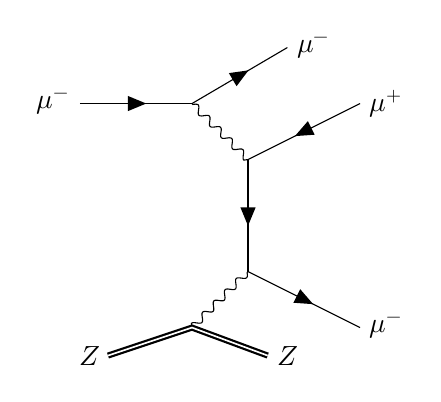
\begin{tikzpicture}
  \centering
   % Sizes
   \pgfmathsetmacro{\len}{0.05cm}
   \pgfmathsetmacro{\halflen}{\len/4}
   \pgfmathsetmacro{\vertexsize}{\len/20}
   \begin{feynman}
       % vertices
       \vertex (a) at (0, 0);
       \vertex (b) at (0, -1*\len);
       \vertex (d) at (-0.5*\len, 0.5*\len);
       \vertex (c) at (-0.5*\len, -1.5*\len);
       \vertex (i1) at (-1.5*\len, 0.5*\len);
       \vertex (i2) at (0, 1.5*\len);
       \vertex (f1) at (\len, 0.5*\len);
       \vertex (f2) at (\len, -1.5*\len);
       \vertex (f3) at (0.5, 1*\len);
       \vertex (z1) at (-1.25*\len, -1.75*\len);
       \vertex (z2) at (0.25, -1.75*\len);
 
       % draw diagram
       \diagram* {
         (i1) -- [fermion] (d) -- [fermion] (f3),
         (d) -- [boson] (a),
         (f1) -- [fermion] (a),
         (a) -- [fermion] (b),
         (b) -- [fermion] (f2),
         (b) -- [boson] (c),
       };
       \draw[thick, double] (z1) -- (c) -- (z2);
 
       % labels
       \node[left] at (i1) {$\mu^-$};
       \node[right] at (f3) {$\mu^-$};
       \node[right] at (f1) {$\mu^+$};
       \node[right] at (f2) {$\mu^-$};
       \node[left] at (z1) {$Z$};
       \node[right] at (z2) {$Z$};
  \end{feynman}
\end{tikzpicture}
    \caption{One possible feynman diagram describing the creation of a muon pair by an ingoing muon.}
    \label{fig:feynman_mupair}
\end{figure}

The process has been described in \cite{Kelner2000} where a simplified analytical double-differential cross section for muon pair production is given by
\begin{equation}
    \label{eqn:mupair}
    \frac{\mathrm{d}^2\sigma}{\mathrm{d}v \mathrm{d}\rho} = \frac{2}{3\pi} (Z \alpha r_\mu)^2 \frac{1-v}{v} \Phi(v, \rho) \ln \left( X \left(E, v, \rho \right) \right)
\end{equation}
with the relative energy loss $v$ and the asymmetry parameter $\rho$ defined by
\begin{align}
    v &= \frac{E_+ + E_-}{E}, & \rho &= \frac{E_+ - E_-}{E_+ + E_-}
\end{align}
and the energy of the produced (anti)muon $E_+$, $E_-$.
The functions $\Phi(v, \rho)$ and $X(E, v, \rho)$ have the form
\begin{align}
    \begin{split}
    \Phi(v, \rho) &= \left[ (2 + \rho^2) (1 + \beta) + \xi (3 + \rho^2) \right] \cdot \ln{ \left( 1 + \frac{1}{\xi} \right) }\\ &+ \left[ (1 + \rho^2) \left( 1 + \frac{3}{2} \beta \right) - \frac{1}{\xi} (1 + 2 \beta) (1 - \rho^2) \right] \cdot \ln{ (1 + \xi) }\\ &- 1 - 3 \rho^2 + \beta (1 - 2 \rho^2)
    \end{split}
\end{align}
where $X$ is given by
\begin{equation}
    X = 1 + U(E, v, \rho) - U(E, v, \rho_\text{max})
\end{equation}
with 
\begin{equation}
    U(E, v, \rho) = \frac{\frac{0.65 m_{\mu}}{m_e} A^{-0.27} B Z^{-\sfrac{1}{3}}}{1 + \frac{2 \sqrt{e} \mu^2 B Z^{-\sfrac{1}{3}} (1 + \xi) (1 + Y) }{m_e E v (1 - \rho^2)} }
\end{equation}
and with 
\begin{align}
    \xi &= \frac{v^2 (1 - \rho^2)}{4 (1 - v)}, & \beta &= \frac{v^2}{2 (1 - v)}, & Y &= 12 \sqrt{\frac{m_{\mu}}{E}}, & B &= 183.
\end{align}

The approximative expression \eqref{eqn:mupair} takes into account the finiteness of the nucleus as well as screening effects of the nucleus by atomic electrons.
A more precise formula for the differential cross section is given in \cite{Kelner2000} as well, however it includes multidimensional integrals that are hard to evaluate and is therefore not suited to be used here.
Furthermore, \eqref{eqn:mupair} is chosen to have a discrepancy compared to the precise formula of below $\SI{10}{\percent}$ for all $E > \SI{e4}{\mega\electronvolt}$, the discrepancy of the derived total cross section is even below $\SI{3}{\percent}$ for $E > \SI{3e4}{\mega\electronvolt}$.

The kinematic limits of the process for $v$ and $\rho$ are
%
\begin{align}
    v_\text{min} &= \frac{2 m_{\mu}}{E}, & v_\text{max} &= 1 - \frac{m}{E}, & \left| \rho \right| \leq \rho_{\text{max}} &= 1 - \frac{2 m_{\mu}}{v E},
\end{align}
%
for an initial particle with mass $m$ and are easy to retrace by demanding the condition that all particles involved have to fulfill $E > m_{\text{rest}}$ at all times.

\subsection{Implementation in PROPOSAL}
\label{sec:mupair_implementation}

% sloppypar is needed here because otherwise \texttt{...} breaks the layout because it cant use hyphenation here
\begin{sloppypar}
The process of muon pair production is implemented as an optional, additional interaction in PROPOSAL.
It is per default disabled in PROPOSAL and can be enabled by setting the keyword \texttt{mupair} in the configuration file to \texttt{MupairKelnerKokoulinPetrukhin} which is the parametrization that has been described in the previous section.
\end{sloppypar}

\begin{sloppypar}
To obtain the single-differential cross section in $v$ from \eqref{eqn:mupair}, a numerical integration across the entire kinematic range of $\rho$
%
\begin{equation}
    \frac{\symup{d}\sigma}{\symup{d}v} = \int_{\rho_{\text{min}}}^{\rho_{\text{max}}} \frac{\mathrm{d}^2\sigma}{\mathrm{d}v \mathrm{d}\rho} \, \symup{d}\rho
\end{equation}
%
is performed in PROPOSAL.
After sampling the relative energy loss $v$ during propagation according to \eqref{eqn:sample_v}, the asymmetry parameter $\rho$ is also sampled if the parameter \texttt{mupair\_particle\_output} has been set to \texttt{True}.
In this case, \eqref{eqn:mupair} is used with a fixed $v = v^{\ast}$ to solve the integral equation
\begin{equation}
    \left( \frac{\symup{d}\sigma}{\symup{d}v}(v^{\ast}) \right)^{-1} \int_{\rho_\text{min}}^{\rho} \frac{\mathrm{d}^2\sigma}{\mathrm{d}v \mathrm{d}\rho}(v^{\ast}) \, \symup{d}\rho = \xi
\end{equation}
for $\rho$ where $\xi \in \left[0,1\right)$ is a random number.
An additional random number is used to decide on the sign of $\rho$, the muon energies then assigned are $E_{\pm} = v E \cdot(1 \pm \rho)$.
In figure \ref{fig:rho_mupair}, the behavior of $\rho$ for different muon energies and different $v$ is shown.
For high energies, the process tends to have a higher asymmetry $\rho$, especially when a high relative energy loss is involved, while for lower energies, lower asymmetries are favored.
\end{sloppypar}

\begin{figure}
    \centering
    \includegraphics[scale=1]{build/mupair_rho.pdf}
    \caption{Histogram of $\lvert\rho\rvert$ for different $v$ of muons in ice. For each $v$, $\rho$ has been sampled $\num{e6}$ times. The dashed curves correspond to an initial muon energy of $E=\SI{e4}{\mega\electronvolt}$, the solid curves to $E = \SI{e9}{\mega\electronvolt}$.}
    \label{fig:rho_mupair}
\end{figure}

A comparison of the average energy loss in ice due to electron-positron pair production and muon pair production is shown in figure \ref{fig:dEdx_mupair}.
Both functions behave similarly as they both grow linearly with $E$, still the contribution from muon pair production is by about three orders of magnitudes lower for higher energies and even lower for small energies.
This observation shows that the process is negligible for the energy loss for the muon which is especially a result of the difference between the muon mass and the electron mass since 
\begin{align*}
	\frac{\sigma_{\mu \text{pair}}}{\sigma_{e \text{pair}}} \propto \frac{r_{\mu}^2}{r_e^2} \propto \frac{m_e^2}{m_{\mu}^2} \propto \num{2e-5}.
\end{align*}

\begin{figure}
    \centering
    \includegraphics[scale=1]{build/dEdx_mupair.pdf}
    \caption{Comparison of the average continuous energy losses of muons in ice due to electron-positron pair production and muon pair production. No energy cuts are applied in this plot, hence this plot represents the case where all losses are treated continuous.}
    \label{fig:dEdx_mupair}
\end{figure}

Figure \ref{fig:spectrum_mupair} shows a secondary particle spectrum where muon pair production is enabled.
The contribution for muon pair production tends to be distributed homogeneously but is, as expected, quantitatively negligible for all secondary energies.

\begin{figure}
    \centering
    \includegraphics[scale=1]{build/spectrum_mupair.pdf}
    \caption{Secondary particle spectrum for $\num{e5}$ muons with an initial energy of $\SI{e8}{\mega\electronvolt}$, propagated in ice. Muon pair production is enabled. The histogram shows the frequency of the stochastic losses during propagation, classified by the type of energy loss. The energy cuts applied here are $e_\text{cut} = \SI{500}{\mega\electronvolt}$, $v_\text{cut} = 0.05$.}
    \label{fig:spectrum_mupair}
\end{figure}

\subsection{Significant detector signatures}
\label{sec:signatures}

As already described and shown in section \ref{sec:mupair_implementation}, the contribution of muon pair production to the overall energy loss of muons is negligible.
However, for detectors interested in muon events, the effects of muon pair production may portray a source of significant signatures.
In the following, a group of muons moving into almost the same direction with only a small separation is called a muon bundle.
The origin of such a bundle can be muon pair production, in this case the bundle consists of three muons.

\subsubsection{IceCube detector}

Due to resolution effects, the IceCube detector is unable to identify the muons in a bundle as individual muon signatures.
However, the signature of a single muon traversing the detector is different from a muon bundle originating from muon pair production with the same sum of energy.
The signature of a high-energetic muon in IceCube is often characterized by a single high-energetic stochastic energy loss creating a spherical signature.
In a muon bundle, each muon with only a fraction of the total energy produces smaller stochastic losses.
Since the stochastic losses of the individual muons in the bundle are independent of each other, the resulting signature is homogeneous and the energy loss per distance of a bundle is more consistent compared to the energy loss per distance of a single muon with the same total energy. \todo{Include an event signature of a high-energetic muon and a muon bundle event? See Tomasz dissertation as a comparison.}

\subsubsection{Underground observatories}

Underground detectors observing muons originating from extensive air showers can use the information about muon bundles created in these air showers to learn about the cosmic ray composition and hadronic interaction models.
This is done by comparing the frequency and multiplicity of muon bundles as well as the muon separation measured in experiments with the predictions from Monte Carlo studies.
In \cite{MupairInRock}, the authors describe this procedure in more detail and point out a possible background from muon pair production.

While about $\SI{1}{\percent}$ to $\SI{10}{\percent}$ of the observed muons are part of muon bundles induced in the air shower, these bundles can also be produced due to muon pair production in rock or water above the underground detector.
According to calculations in \cite{MupairInRock}, these bundles induced by muon pair production can portray a background of up to $\SI{10}{\percent}$ compared to the conventional bundles in the showers, although more exact calculations have to be performed individually for each experiment with its own geometric properties.
Due to the difference in the distance between the creation and observation point of the muon bundle, both effects can be separated statistically by examining the separation distance in the bundle.
The separation of muon bundles due to muon pair production is mostly below $\SI{1}{\metre}$ while for muon bundles induced in air showers, only a small percentage of the muon bundles have such a small separation \cite{MupairInRock}.

\section{Weak interaction of charged leptons}

The process called weak interaction in PROPOSAL refers to the conversion of a charged lepton to a neutrino under exchange of a $W$-boson, i.e.\ a charged current weak interaction.
This interaction is highly suppressed compared to other processes, its signature however can be of importance, for example as a background for tau neutrino searches as described in section \ref{sec:weak_signature}.

\subsection{Theory and description of the data}
\label{sec:weak_theory}

The process of interest
%
\begin{equation}
    \label{eqn:weak_lepton}
    l + N \rightarrow \nu_l + X
\end{equation}
%
with a charged lepton $l$, the corresponding neutrino $\nu_l$, the initial nucleon $N$ and the hadronic final state $X$ describes the conversion of a charged lepton to a neutrino under exchange of a $W$-boson.
This specific process is related to the interaction of an anti-neutrino under exchange of a $W$ boson, i.e.\
%
\begin{equation}
    \label{eqn:weak_neutrino}
    \overline{\nu}_l + N \rightarrow \overline{l} + X,
\end{equation}
%
via crossing symmetry\footnote{The argument of crossing symmetry is identical when switching all particles with their corresponding antiparticles, i.e.\ the process $\overline{l} + N \rightarrow \overline{\nu}_l + X$ is connected to $\nu_l + N \rightarrow l + X$.} as depicted in figure \ref{fig:feynman_weak}.
%
\begin{figure}
    \centering
    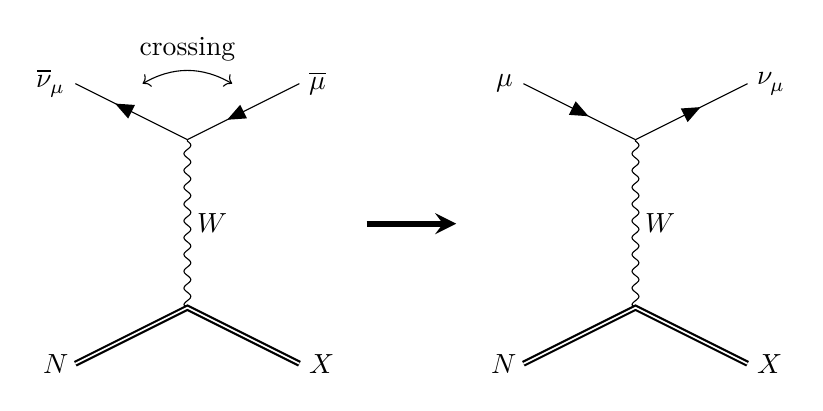
\begin{tikzpicture}
  \centering
   % Sizes
   \pgfmathsetmacro{\len}{0.05cm}
   \pgfmathsetmacro{\halflen}{\len/4}
   \pgfmathsetmacro{\vertexsize}{\len/20}
   \begin{feynman}
       % vertices
       \vertex (a) at (-1*\len, 0.5*\len);
       \vertex (b) at (0, 0);
       \vertex (c) at (1*\len, 0.5*\len);
       \vertex (d) at (0, -1.5*\len);
       \vertex (e) at (-1*\len, -2*\len);
       \vertex (f) at (1*\len, -2*\len);

       \vertex (x) at (-0.4*\len, 0.5*\len);
       \vertex (y) at ( 0.4*\len, 0.5*\len); 
  
       % draw diagram
       \diagram* {
         (a) -- [anti fermion] (b) -- [anti fermion] (c),
         (b) -- [boson, edge label=\(W\)] (d),

       };
       \draw[thick, double] (e) -- (d) -- (f);
  
       \path[] (x) edge[<->, bend left] node [above] {crossing} (y);

       % labels
       \node[left] at (a) {$\overline{\nu}_{\mu}$};
       \node[right] at (c) {$\overline{\mu}$};
       \node[left] at (e) {$N$};
       \node[right] at (f) {$X$};

       % arrow inbetween

       \vertex (i1) at (1.6*\len, -0.75*\len);
       \vertex (i2) at (2.4*\len, -0.75*\len);
       \path[line width=0.8mm, black, ->, >=stealth] (i1) edge[->] node [] {} (i2);

       % vertices second diagram
       \vertex (a2) at (4*\len -1*\len, 0.5*\len);
       \vertex (b2) at (4*\len + 0, 0);
       \vertex (c2) at (4*\len + 1*\len, 0.5*\len);
       \vertex (d2) at (4*\len + 0, -1.5*\len);
       \vertex (e2) at (4*\len -1*\len, -2*\len);
       \vertex (f2) at (4*\len + 1*\len, -2*\len);
  
       % draw second diagram
       \diagram* {
         (a2) -- [fermion] (b2) -- [fermion] (c2),
         (b2) -- [boson, edge label=\(W\)] (d2),

       };
       \draw[thick, double] (e2) -- (d2) -- (f2);
  
       % labels second diagram
       \node[left] at (a2) {$\mu$};
       \node[right] at (c2) {$\nu_{\mu}$};
       \node[left] at (e2) {$N$};
       \node[right] at (f2) {$X$};

  \end{feynman}
\end{tikzpicture}
    \caption{Feynman diagrams of lepton interactions under exchange of a $W$-boson and its connection via crossing symmetry.}
    \label{fig:feynman_weak}
\end{figure}
%
Since the kinematics of both processes are identical, the differential cross sections are also identical except for a prefactor of $\sfrac{1}{2}$,
%
\begin{equation}
    \symup{d}\sigma\left( l + N \rightarrow \nu_l + X \right) = \frac{1}{2} \symup{d}\sigma\left( \overline{\nu}_l + N \rightarrow \overline{l} + X \right).
\end{equation}
%
Due to averaging over all possible initial states and summing over all possible final states when evaluating feynman diagrams, the prefactor $\sfrac{1}{2}$ must be taken into account since the muon can both be left-handed and right-handed while neutrinos are only observed in a left-handed state (and antineutrinos in a right-handed state).

Data on the differential cross section for the conversion of a neutrino to a charged lepton, i.e.\ the process \eqref{eqn:weak_neutrino}, are available from \cite{Cooper_Sarkar_2011}.
By using crossing symmetry, these data can directly be used to describe the conversion of a charged lepton to a neutrino, i.e.\ \eqref{eqn:weak_lepton}, which is the process of interest in PROPOSAL.

The cross sections for interactions of leptons with hadrons can be derived under the use of parton distribution functions which describe the probability to find a specific parton (quark or gluon) with a given fraction $x$ of the nucleon's momentum when the momentum transfer is given by $Q^2$.
To make predictions for the (anti)neutrino charged current cross sections, \cite{Cooper_Sarkar_2011} performs next-to-leading order calculations and uses the HERAPDF1.5 data set which provides the parton distribution functions based on deep-inelastic scattering measurements performed from 2003 to 2007 at the HERA experiment \cite{am2010proton}.

The values for $\sfrac{\symup{d}\sigma}{\symup{d}v}$ are provided as two-dimensional tables in $E$ and $v$ with $\num{100}$ entries in $E$ and, for each energy, $\num{110}$ entires in $v$.  
Here, $v$ describes the fraction of the initial lepton energy $E$ lost to the nucleon.
Tables are available for an ingoing neutrino or an ingoing antineutrino and for a proton or a neutron as a nucleon involved in the interaction.
The ranges are $\SI{10}{\giga\electronvolt} \leq E \leq \SI{e12}{\giga\electronvolt}$ and $v_\text{min} < v < 1$ with logarithmic steps in between where the lower limit of $v$ has been set to
%
\begin{align}
    v_\text{min} &= \frac{Q^2_{\text{min}}}{s}, & s &= 2 E m + m^2, & Q^2_{\text{min}} &= \SI{1}{\giga\electronvolt^2}
\end{align}
%
with the mass of the involved nucleon $m$ and the center-of-mass energy $\sqrt{s}$.
For values where $Q^2 < Q_\text{min}^2$, the underlying theory of quantum chromodynamics can not be treated perturbatively anymore, meaning that the predictions for the cross sections are not reliable in this kinematic range. 

\subsection{Implementation in PROPOSAL}
\label{sec:weak_implementation}

% sloppypar is needed here because otherwise \texttt{...} breaks the layout because it cant use hyphenation here
\begin{sloppypar}
The weak interaction process is by default disabled in PROPOSAL and can optionally be enabled by setting the keyword \texttt{weak} in the configuration file to \texttt{CooperSarkarMertsch} which is the parametrization described in the previous section.
\end{sloppypar}
For a component with an atomic number $Z$ and a mass number $A$, the differential cross section is combined from the given tables to be
%
\begin{equation}
	\frac{\symup{d}\sigma}{\symup{d}v} \propto Z \cdot \frac{\symup{d}\sigma_p}{\symup{d}v} + (A - Z) \cdot \frac{\symup{d}\sigma_n}{\symup{d}v}
\end{equation}
%
where the subscript refers to the nucleon involved in the interaction ($p$ for proton and $n$ for neutron).
PROPOSAL then uses a two-dimensional interpolation routine to obtain a continuous differential cross section from the discrete tables values.

In contrast to previously described processes, the weak interaction is a catastrophic loss meaning that the initial particle ceases to exist since it is converted to a different type of particle during the interaction.
Treating a process with this signature continuously as described in section \ref{sec:energy_loss_calculation} would therefore be unphysical.
Instead, all interactions with catastrophic losses are treated stochastically by setting $v_{\text{min}} = v_{\text{cut}}$ in \eqref{eqn:fE}, \eqref{eqn:stoch_crosssection} and \eqref{eqn:sample_v}.
Afterwards, PROPOSAL returns the produced neutrino as well as the energy transfer to the nucleon and stops the particle propagation.

\begin{figure}
    \centering
    \includegraphics[scale=1]{build/dNdx_weak.pdf}
    \caption{Comparison of the stochastic cross sections for muons in ice for weak interaction in comparison to other interactions. The cut settings are set to $e_\text{cut} = \SI{500}{\mega\electronvolt}$, $v_\text{cut} = 0.05$. Note that the weak interaction cross section is not affected by the cut settings.}
    \label{fig:dNdx_weak}
\end{figure}

Figure \ref{fig:dNdx_weak} shows the weak interaction cross section of muons in ice compared to the total stochastic cross section of default processes.
It is important to note for this comparison that, while $v_{\text{min}} = v_{\text{cut}}$ is used for the weak interaction, a regular energy cut of $e_\text{cut} = \SI{500}{\mega\electronvolt}$ and $v_\text{cut} = 0.05$ is still used for the other parametrizations.
Still, it becomes obvious that the weak interaction is a strongly suppressed process compared to all other interactions.

\subsection{Significant detector signatures}
\label{sec:weak_signature}

As described in the previous section, the weak interaction process is highly suppressed and therefore negligible in its contribution to the energy loss of a charged lepton.
However, under certain conditions, the detector signature of the process could be significant for searches of tau neutrinos, for example in the IceCube neutrino observatory.

\begin{figure}
    \centering
    \begin{subfigure}{0.46\textwidth}
        \centering
        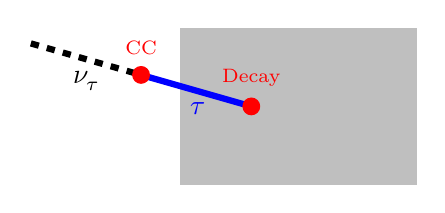
\begin{tikzpicture}
	\centering
	\fill [lightgray] (0.0, 0.0) rectangle (3.0, 2.0);
	\draw [line width=0.8mm, blue] (-0.5, 1.4) -- node[below] {$\tau$}  (0.9, 1.);
	\draw [line width=0.8mm, black, dashed] (-1.9, 1.8) -- node[below] {$\nu_{\tau}$}  (-0.5, 1.4);
	\draw[red,fill=red] (0.9, 1.) circle (0.7ex) node[label=above: $\scriptsize \text{Decay}$]{};
	\draw[red,fill=red] (-0.5, 1.4) circle (0.7ex) node[label=above: $\scriptsize \text{CC}$]{};
\end{tikzpicture} 

        \caption{Lollipop signature triggered by a tau neutrino.}
        \label{fig:lollipop_signature}
    \end{subfigure}%
    \hspace{0.06\textwidth}%
    \begin{subfigure}{0.46\textwidth}
        \centering
        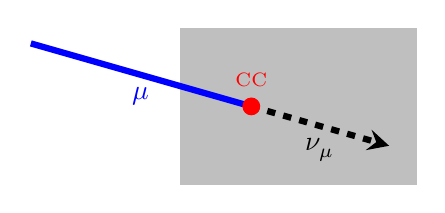
\begin{tikzpicture}
	\centering 
	\fill [lightgray] (0.0, 0.0) rectangle (3.0, 2.0);
	\draw [line width=0.8mm, blue] (-1.9, 1.8) -- node[below] {$\mu$}  (0.9, 1.);
	\draw [line width=0.8mm, black, dashed, ->, >=stealth] (0.9, 1.) -- node[below] {$\nu_{\mu}$}  (0.9+1.4+0.35, 1. - 0.4 - 0.1);
	\draw[red,fill=red] (0.9, 1.) circle (0.7ex) node[label=above: $\scriptsize \text{CC}$]{};
\end{tikzpicture} 

        \caption{Signature of a muon weakly interacting inside the detector.}
        \label{fig:weak_signature}
    \end{subfigure}
    \caption{Illustrations of two signatures relevant for tau neutrino searches. The detector volume is drawn gray, hadronic cascades are drawn as a red dot, observable tracks are drawn as blue lines and tracks that are not directly observable are drawn as a black, dotted line.}
    \label{fig:test}
\end{figure}

One possible signature hinting at a tau neutrino event called the "lollipop" signature is illustrated in figure \ref{fig:lollipop_signature}.
Here, a tau neutrino moving towards the detector interacts via a charged current before it reaches the detector and is being converted to a tau lepton.
The tau lepton then enters the detector, leaving behind an observable track of Cherenkov light emerging from the tau itself and the created secondary particles.
Due to its short lifetime, the created tau can only reach the detector if its energy is high enough, the average tau decay length scales with energy as \SI{5}{\cm\per\tera\electronvolt} \cite{Aartsen_2016} meaning the tau energy has to be $E_{\tau} \gtrapprox \SI{100}{\tera\electronvolt}$.
If the tau decays to a hadron inside the detector, a hadronic cascade is generated at the end of the track, giving the signature its characteristic name. 

This tau neutrino signature can be imitated by the event shown in figure \ref{fig:weak_signature}.
In this case, a muon, leaving behind a track, enters the detector where it weakly interacts and is therefore converted to a neutrino.
Due to the energy transfer to the involved nucleus in the weak interaction, the process creates a hadronic cascade comparable to the cascade of a hadronic tau decay.
Since the created neutrino is not observable, the overall signature where a track starts outside the detector and ends in a hadronic cascade can be confused with the lollipop signature from figure \ref{fig:lollipop_signature}.
However, the tracks from both signatures behave differently since the energy loss per distance of a muon is higher than the energy loss of a tau.
To have a similar track signature, the tau involved needs to have an energy that is about $\num{6}$ to $\num{11}$ times higher than the energy of a corresponding muon \cite{Sandrock:2018hpj}.

It follows that analyses searching for lollipop signatures have to consider the weak interaction as a possible background.
According to approximative calculations in \cite{Sandrock:2018hpj} based on the properties of the IceCube detector, the expected rate of false lollipop events due to atmospheric muons undergoing weak interaction is about $\SI{2e-2}{\per yr}$. 
This, together with further approximative calculations for real lollipop signatures from tau neutrino events, corresponds to a possible background of $\SI{10}{\percent}$.
However, further effects such as event selection efficiency (assumed to be perfect in this calculation) or a detailed detector simulation were not taken into account but need to be evaluated when conducting a detailed analysis.

\chapter{Propagation of electromagnetic showers}

\section{Electron and positron propagation in PROPOSAL}

\label{sec:electronprop}

\subsection{Ionization}

Ionization describes the inelastic collision of a particle with atomic electrons, leading to an energy loss of the primary particle.
For heavy, charged particles the average energy loss due to ionization is given by the Bethe formula.
PROPOSAL uses a modified Bethe formula, taking into account density correction effects, to describe the ionization losses for muons and tau particles \cite{Kohne:2013zbq}.
However, the Bethe formula can't be applied for electrons and positrons due to their lower mass as well as the indistinguishability of incoming electrons with atomic electrons.
Therefore, a separate treatment of the ionization losses for electrons and positrons is necessary.

\subsubsection{Theoretical description}

For energy transfers $\nu$ significantly greater than the atomic excitation levels, the atomic electrons can be considered as free and in rest.
In this case, the ionization process is essentially electron-electron scattering ($e^- + e^- \rightarrow e^- + e^-$), known as M{\o}ller scattering, or positron-electron scattering ($e^+ + e^- \rightarrow e^+ + e^-$), known as Bhabha scattering.
The two feynman diagrams contributing in leading order for M{\o}ller scattering are shown in figure \ref{fig:feynman_moller}, the differential cross section \cite{PhysRev.93.38} is given by
%
\begin{equation}
	\begin{split}
	\label{eqn:moller}
	\left(\frac{\symup{d}\sigma}{\symup{d}v}\right)_{\!\!-} &= \frac{2 \pi r_e^2 Z \gamma}{\beta^2(\gamma - 1)^2} \biggl[ \frac{(\gamma - 1)^2}{\gamma^2} + \frac{1}{\epsilon} \left( \frac{1}{\epsilon} - \frac{2\gamma - 1}{\gamma^2} \right) \\ &\quad+ \frac{1}{1 - \epsilon} \left( \frac{1}{1 - \epsilon} - \frac{2 \gamma - 1}{\gamma^2} \right) \biggr]
	\end{split}
\end{equation}
%
with
%
\begin{align}
	\epsilon &= \frac{v E}{E - m_e},& \gamma &= \frac{E}{m_e}, & \beta &= \sqrt{1 - \frac{1}{\gamma^2}}, & v_{\text{max}} = \frac{1}{2} - \frac{m_e}{2 E}.
\end{align}

\begin{figure}
    \centering
    \begin{tikzpicture}
  \centering
   % Sizes
   \pgfmathsetmacro{\len}{0.05cm}
   \pgfmathsetmacro{\halflen}{\len/4}
   \pgfmathsetmacro{\vertexsize}{\len/20}
   \begin{feynman}
       % vertices
       \vertex (a) at (-1*\len, 0.5*\len);
       \vertex (b) at (0, 0);
       \vertex (c) at (1*\len, 0.5*\len);
       \vertex (d) at (0, -1.5*\len);
       \vertex (e) at (-1*\len, -2*\len);
       \vertex (f) at (1*\len, -2*\len);
  
       \vertex [label=\(\gamma\)] (label) at (-0.3 , -0.9 * \len);

       % draw diagram
       \diagram* {
         (a) -- [fermion] (b) -- [fermion] (c),
         (b) -- [photon] (d),
         (e) -- [fermion] (d) -- [fermion] (f)
       };  
       % labels
       \node[left] at (a) {$e^-$};
       \node[right] at (c) {$e^-$};
       \node[left] at (e) {$e^-$};
       \node[right] at (f) {$e^-$};

       % vertices
       \vertex (a2) at (6-1*\len, 0.5*\len);
       \vertex (b2) at (6+0, 0);
       \vertex (f2) at (6+1*\len, 0.5*\len);
       \vertex (d2) at (6+0, -1.5*\len);
       \vertex (e2) at (6-1*\len, -2*\len);
       \vertex (c2) at (6+1*\len, -2*\len);

       \vertex [label=\(\gamma\)] (label2) at (6-0.3 , -0.9 * \len);
  
       % draw diagram
       \diagram* {
         (a2) -- [fermion] (b2) -- [fermion] (c2),
         (b2) -- [photon] (d2),
         (e2) -- [fermion] (d2) -- [fermion] (f2)
       };  
       % labels
       \node[left] at (a2) {$e^-$};
       \node[right] at (c2) {$e^-$};
       \node[left] at (e2) {$e^-$};
       \node[right] at (f2) {$e^-$};


  \end{feynman}
\end{tikzpicture}
    \caption{Feynman diagrams in leading order for M{\o}ller scattering. The $t$-channel diagram is shown on the left, the $u$-channel diagram is shown on the right.}
    \label{fig:feynman_moller}
\end{figure}

For Bhabha scattering, the two feynman diagrams contributing in leading order are shown in figure \ref{fig:feynman_bhabha} and the differential cross section \cite{PhysRev.93.38} is given by
%
\begin{equation}
	\label{eqn:bhabha}
	\left(\frac{\symup{d}\sigma}{\symup{d}v}\right)_{\!\!+} = \frac{2 \pi r_e^2 Z \gamma}{(\gamma - 1)^2} \left[ \frac{1}{\beta^2 \epsilon^2} - \frac{B_1}{\epsilon} + B_2 - B_3 \epsilon + B_4 \epsilon^2 \right]
\end{equation}
%
with
%
\begin{align*}
	B_1 &= 2 - y^2, & B_2 &= (1 - 2y)(3 + y^2), \\ 
	B_3 &= (1-2y)^2 + (1 - 2y)^3, & B_4 &= (1 - 2y)^3 \\
	\intertext{and}
	y &= \frac{1}{\gamma + 1}, & v_{\text{max}} &= 1 - \frac{m_e}{E}.
\end{align*}

\begin{figure}
    \centering
    \begin{tikzpicture}
  \centering
   % Sizes
   \pgfmathsetmacro{\len}{0.05cm}
   \pgfmathsetmacro{\halflen}{\len/4}
   \pgfmathsetmacro{\vertexsize}{\len/20}
   \begin{feynman}
       % vertices
       \vertex (a) at (-1*\len, 0.5*\len);
       \vertex (b) at (0, 0);
       \vertex (c) at (1*\len, 0.5*\len);
       \vertex (d) at (0, -1.5*\len);
       \vertex (e) at (-1*\len, -2*\len);
       \vertex (f) at (1*\len, -2*\len);
  
       \vertex [label=\(\gamma\)] (label) at (-0.3 , -0.9 * \len);

       % draw diagram
       \diagram* {
         (a) -- [anti fermion] (b) -- [anti fermion] (c),
         (b) -- [photon] (d),
         (e) -- [fermion] (d) -- [fermion] (f)
       };  
       % labels
       \node[left] at (a) {$e^+$};
       \node[right] at (c) {$e^+$};
       \node[left] at (e) {$e^-$};
       \node[right] at (f) {$e^-$};

       % vertices
       \vertex (a2) at (6-1*\len, 0.5*\len);
       \vertex (b2) at (6-0.5, -0.75*\len);
       \vertex (f2) at (6+1*\len, 0.5*\len);
       \vertex (d2) at (6+0.5, -0.75*\len);
       \vertex (e2) at (6-1*\len, -2*\len);
       \vertex (c2) at (6+1*\len, -2*\len);
  
       % draw diagram
       \diagram* {
         (a2) -- [anti fermion] (b2) -- [anti fermion] (e2),
         (b2) -- [photon, edge label=\(\gamma\)] (d2),
         (c2) -- [anti fermion] (d2) -- [anti fermion] (f2)
       };  
       % labels
       \node[left] at (a2) {$e^+$};
       \node[right] at (c2) {$e^-$};
       \node[left] at (e2) {$e^-$};
       \node[right] at (f2) {$e^+$};


  \end{feynman}
\end{tikzpicture}
    \caption{Feynman diagrams in leading order for Bhabha scattering. The diagram describing the scattering process is shown on the left, the diagram describing the annihilation process is shown on the right.}
    \label{fig:feynman_bhabha}
\end{figure}

For energy transfers $\nu$ in the same order of magnitude as the atomic excitation levels, the explicit excitation probabilities $p(E, v)$ need to be considered.
Defining a threshold transfer energy $\nu_{\text{thres}}$ that is above the atomic excitation levels but below the energy cut in PROPOSAL, the continuous energy loss per distance due to ionization can be written as
%
\begin{equation}
	\label{eqn:ioniz_sum}
	-\left(\frac{\symup{d}E}{\symup{d}X}\right)_{\!\!\pm} \propto \int_{0}^{\sfrac{\nu_{\text{thres}}}{E}} v \cdot p(E, v) \, \symup{d}v + \int_{\sfrac{\nu_{\text{thres}}}{E}}^{v_{\text{cut}}} v \cdot \left(\frac{\symup{d}\sigma}{\symup{d}v}\right)_{\!\!\pm} \, \symup{d}v. 
\end{equation}
%
For an appropriate value of $\nu_{\text{thres}}$, certain approximations can be applied where \eqref{eqn:ioniz_sum} yields
%
\begin{equation}
	- \left(\frac{\symup{d}E}{\symup{d}X}\right)_{\!\!\pm} = \frac{2 \pi r_e^2 m_e}{\beta^2} \left[ \log{\left( \frac{2 m_e (\tau + 2)}{I} \right) + F^{\pm}(\tau, \Delta) - \delta } \right],
\end{equation}
%
also known as the Berger-Seltzer formula \cite{Hirayama:2005zm}, with
%
\begin{align}
	\tau &= \gamma - 1, & \Delta = \text{min}\left[ \frac{v_{\text{max}} E}{m_e}, \frac{v_{\text{cut}} E}{m_e} \right],
\end{align}
%
the mean ionization energy of the medium $I$ and the contribution from the density correction $\delta$ described in detail in \cite{Kohne:2013zbq}.
Furthermore, $F^{\pm}(\tau, \Delta)$ differs for electrons and positrons and is defined by
\begin{align}
	\begin{split}
	F^{+}(\tau, \Delta) &= \ln\left(\tau \Delta \right) - \frac{\beta^2}{\tau} \biggl[ \tau + 2 \Delta - \frac{3 \Delta^2 }{2} \\ &\quad- (\Delta - \frac{\Delta^2}{3}) y^2 - ( \frac{\Delta^2}{2} - \frac{\tau\Delta^3}{3} + \frac{\Delta^4}{4} ) y^3 \biggr],
	\end{split}
	\\[2ex]
	\begin{split}
	F^{-}(\tau, \Delta) &= -1 - \beta^2 + \ln\left( (\tau - \Delta) \Delta \right) + \frac{\tau}{\tau - \Delta} \\ &\quad+ \frac{1}{\gamma^2} \left[ \frac{\Delta^2}{2} + (2 \tau + 1) \log\left( 1 - \frac{\Delta}{\tau} \right) \right].
	\end{split}
\end{align}

\subsubsection{Implementation in PROPOSAL}


% sloppypar is needed here because otherwise \texttt{...} breaks the layout because it cant use hyphenation here
\begin{sloppypar}
The ionization cross sections for electrons and positrons described above can be used in PROPOSAL by setting the keyword \texttt{ioniz} in the configuration file to \texttt{IonizBergerSeltzerMoller} to use the parametrization for electrons or \texttt{IonizBergerSeltzerBhabha} to use the parametrization for positrons. 
\end{sloppypar}

To take into account the atomic excitation levels relevant for small energy transfers, the Berger-Seltzer formula, i.e.\ \eqref{eqn:ioniz_sum}, is used when calculating the continuous ionization losses.
When sampling the stochastic losses the differential cross section for M{\o}ller scattering \eqref{eqn:moller}, respectively the differential cross section for Bhabha scattering \eqref{eqn:bhabha}, is used directly since the contributions from small energy transfers are negligible here.

Figure \ref{fig:dEdx_ionization} shows the differences in the continuous ionization loss for electrons and positrons when using the appropriate Berger-Seltzer formula compared to the Bethe formula.
It can be seen that the influence is up to $\SI{20}{\percent}$ for high energies.
%
\begin{figure}
    \centering
    \includegraphics[scale=1]{build/dEdx_ionization.pdf}
    \caption{Average energy loss of electrons and positrons in air due to ionization. Note that the Bethe formula is, unlike the Berger-Seltzer formula, identical for electrons and positrons.}
    \label{fig:dEdx_ionization}
\end{figure}
%
Furthermore, the Berger-Seltzer formula, compared to the Bethe formula which is independent of the particle charge, differentiates between electrons and positrons.
While the contribution from the atomic excitation levels is, as a good approximation, identical for electrons and positrons, the contribution from high energy transfers differs.
Here, if the ingoing particle is an electron, it is indistinguishable from the atomic electron after the ionization process.
Therefore, the electron with the higher energy after the interaction is by definition the initial particle.
A positron as an ingoing particle however is always distinguishable from the atomic electron and can therefore be the particle with the lower energy after the interaction.

\subsection{Bremsstrahlung}

Bremsstrahlung describes the energy loss of a charged particle in the field of an atomic nucleus $Z$ where a photon is emitted, i.e.\
%
\begin{align*}
	e^{\pm} + Z \rightarrow e^{\pm} + Z + \gamma.
\end{align*}
%
Since the process has a $m^{-2}$ mass dependency, bremsstrahlung is the dominant interaction for high energy electrons and positrons.
It is therefore relevant to provide an accurate description of the bremsstrahlung cross section.

For electrons with high energies, \cite{Kohne:2013zbq} recommends the usage of the Complete Screening parametrization which has already been implemented in PROPOSAL.
This ultra-relativistic cross section, given and described by \cite{RevModPhys.46.815}, uses Coulomb corrections as well as the assumption that the screening of the Coulomb field of the nucleus by the atomic electron cloud is maximal, which is an appropriate approximation for high-energy electrons.

EGS uses an alternative parametrization of the bremsstrahlung interaction, including empirical corrections for low energies.
This parametrization is implemented in PROPOSAL to examine the differences between the cross sections provided by PROPOSAL and EGS as well as the influence from the low energy corrections.

\subsubsection{Theoretical description}

The bremsstrahlung cross section provided by EGS5, which is described in detail by \cite{Hirayama:2005zm}, is split into a high-energy and a low-energy part with a discrete cut at $\SI{50}{\mega\electronvolt}$.

For $E > \SI{50}{\mega\electronvolt}$, the ultra-relativistic differential cross section, comparable to the Complete Screening parametrization in PROPOSAL, is given by
%
\begin{equation}
	\label{eqn:brems_high}
	\begin{split}
	\frac{\symup{d}\sigma}{\symup{d}v} &= \frac{Z (Z + \xi(Z)) r_e^2 \alpha}{v} \biggl[ (2 - 2 v + v^2) \left( \Phi_1(x) - \frac{4}{3} \ln(Z) - 4 f_c(Z) \right) \\ &\quad- \frac{2}{3} (1 - v) \left( \Phi_2(x) - \frac{4}{3} \ln(Z) - 4 f_c(Z) \right) \biggl]
	\end{split}
\end{equation}
%
with
%
\begin{align}
	x &= 136 Z^{-\sfrac{1}{3}} \frac{2 \delta}{m_e}, & \delta &= \frac{m_e^2 v}{2 E (1 - v)}.
\end{align}
%
The functions $\Phi_1(x)$, $\Phi_2(x)$ describe the screening effects and are given by
%
\begin{align}
	\Phi_1(x) &= 
	\begin{cases}
		20.867 - 3.242 x + 0.625 x^2 & \text{if $x \leq 1$},\\
		21.12 - 4.184 \ln(x + 0.952) & \text{if $x > 1$},\\
	\end{cases}\\
	\Phi_2(x) &= 
	\begin{cases}
		20.029 - 1.930 x - 0.086 x^2 & \text{if $x \leq 1$},\\
		21.12 - 4.184 \ln(x + 0.952) & \text{if $x > 1$},\\
	\end{cases}
\end{align}
%
which is an analytical approximation of the Thomas-Fermi form factors.
Furthermore, $f_c(Z)$ describes the Coulomb correction and is approximated in an analytical form by
%
\begin{equation}
	f_c(Z) \approx a^2 \left[ \frac{1}{1 + a^2} + 0.20206 - 0.0369a^2 + 0.0083 a^4 - 0.002 a^6 \right]
\end{equation}
%
with $a = \alpha Z$.
The parameter 
%
\begin{equation}
	\xi(Z) = \frac{L_\text{rad}^{\prime}(Z)}{L_\text{rad}(Z) - f_c(Z)} 
\end{equation}
%
accounts for atomic electron effects where the radiation logarithms are given by
\begin{align}
	L_\text{rad}^{\prime} &=
	\begin{cases}
		\ln(1194 Z^{-\sfrac{2}{3}}) & \text{if $Z > 4$}, \\
		5.924 & \text{if $Z = 4$}, \\
		5.805 & \text{if $Z = 3$}, \\
		5.621 & \text{if $Z = 2$}, \\
		6.144 & \text{if $Z = 1$},
	\end{cases} \\
	L_\text{rad} &=
	\begin{cases}
		\ln(184.15 Z^{-\sfrac{1}{3}}) & \text{if $Z > 4$}, \\
		4.710 & \text{if $Z = 4$}, \\
		4.740 & \text{if $Z = 3$}, \\
		4.790 & \text{if $Z = 2$}, \\
		5.310 & \text{if $Z = 1$}.
	\end{cases}
\end{align}

For $E < \SI{50}{\mega\electronvolt}$, the differential bremsstrahlung cross section is given by
%
\begin{equation}
	\label{eqn:brems_low}
	\begin{split}
	\frac{\symup{d}\sigma}{\symup{d}v} &= \frac{A^{\prime}(E, Z) Z (Z + \xi(Z)) r_e^2 \alpha}{v} \biggl[ (2 - 2 v + v^2) \left( \Phi_1(x) - \frac{4}{3} \ln(Z) \right) \\ &\quad- \frac{2}{3} (1 - v) \left( \Phi_2(x) - \frac{4}{3} \ln(Z) \right) \biggl]
	\end{split}	
\end{equation}
%
where a density correction factor $A^{\prime}(E,Z)$ has been introduced.
This factor $A^{\prime}(E,Z)$ rescales the differential cross section to be in agreement with the empirical average energy losses per distance from \cite{icru37}, the detailed procedure to obtain this correction is described in \cite{pirs}.
It should be noted that this factor is only a normalization factor and is therefore not affecting the shape of the energy loss distribution itself.

\subsubsection{Implementation in PROPOSAL}

% sloppypar is needed here because otherwise \texttt{...} breaks the layout because it cant use hyphenation here
\begin{sloppypar}
To use the bremsstrahlung cross section described above in PROPOSAL, the keyword \texttt{brems} in the configuration file can be set to \texttt{BremsElectronScreening}.
\end{sloppypar}

The values for $A^{\prime}(E,Z)$ are provided as a two-dimensional table in $\ln(Z)$ and $E$ with $\num{14}$ entries in $\ln(Z)$ and, for each $\ln(Z)$, $\num{115}$ entires in $E$.  
PROPOSAL uses a two-dimensional interpolation routine to obtain the correction factor for an arbitrary $Z$, $E$ from the discrete tables values.

\begin{figure}
    \centering
    \includegraphics[scale=1]{build/dEdx_brems.pdf}
    \caption{Comparison of the average energy loss of electrons in air due to bremsstrahlung between the parametrization adapted from EGS (Electron Screening) and two alternative parametrizations (Complete Screening, Andreev Bezrukov Bugaev). The dashed red line highlights the cut applied in the Electron Screening parametrization between the high-energy and low-energy part.}
    \label{fig:dEdx_brems}
\end{figure}


Figure \ref{fig:dEdx_brems} shows a comparison of the average energy loss for electrons\footnote{The bremsstrahlung cross section is identical for positrons which is valid regarding lowest order calculations in $\alpha$ \cite{RevModPhys.46.815}.} loss due to bremsstrahlung when using different differential cross sections.
For very high energies, all parametrizations yield comparable results.
However, differences exceeding a factor of $\num{1.5}$ can be seen for lower energies, especially in the domain of several \si{\mega\electronvolt}.
It is particularly noticeable that the results from the Electron Screening parametrization are in better agreement with the Andreev Bezrukov Bugaev parametrization than the Complete Screening parametrization, although the latter has been recommended for (high) electron electrons.

Furthermore, a discontinuity at $\SI{50}{\mega\electronvolt}$ when using the Electron Screening parametrization is notable.
This behavior results from the fact that the correction factor $A^{\prime}(E,Z)$ is set to $1$ for $E > \SI{50}{\mega\electronvolt}$ although this approximation is invalid according to the empirical data which imply that $A^{\prime}(E,Z) \neq 1$ for energies above the cut.
A smoothing of the correction parameter around $\SI{50}{\mega\electronvolt}$ could remove the unphysical discontinuity, however, such a method would be arbitrary to a certain extend.
Alternatively, using a differential cross section applicable for all energies without relying on empirical correction factors would be preferable for PROPOSAL. 

\subsection{Electron-positron annihilation}
\label{sec:annihilation}
\subsubsection{Theoretical description}

Electron-positron annihilation, only called annihilation in the further course of this section, describes the collision of a positron with an atomic electron where both particles annihilate and a pair of photons is created, i.e\ the process
%
\begin{align*}
	e^+ + e^- \rightarrow \gamma + \gamma,
\end{align*}
which is therefore only relevant when propagating positrons.
%
The feynman diagram describing this process in leading order is shown in figure \ref{fig:feynman_annihilation}.
%
\begin{figure}
    \centering
    \begin{tikzpicture}
  \centering
   % Sizes
   \pgfmathsetmacro{\len}{0.05cm}
   \pgfmathsetmacro{\halflen}{\len/4}
   \pgfmathsetmacro{\vertexsize}{\len/20}
   \begin{feynman}
       % vertices
       \vertex (c) at (0, 0);
       \vertex (b) at (0, -1.5*\len);
       \vertex (a) at (-1*\len, -2*\len);
       \vertex (f) at (+1*\len, -2*\len);
       \vertex (d) at (-1*\len, 0.5*\len);
       \vertex (e) at (+1*\len, 0.5*\len);
 
       % draw diagram
       \diagram* {
         (a) -- [fermion] (b) -- [fermion] (c) -- [fermion] (d),
         (c) -- [boson, edge label=\(\gamma\)] (e),
         (b) -- [boson, edge label=\(\gamma\)] (f)
       };

       % labels
       \node[left] at (d) {$e^+$};
       \node[left] at (a) {$e^-$};
  \end{feynman}
\end{tikzpicture} 

    \caption{Feynman diagram in leading order for electron-positron annihilation.}
    \label{fig:feynman_annihilation}
\end{figure}

Under the assumption that the atomic electron is initially free and at rest, which is a good approximation for positrons with energies high compared to atomic binding energies, the differential annihilation cross section is described by the Heitler formula \cite{heitler1954quantum} given by \cite{Hirayama:2005zm}
%
\begin{equation}
	\label{eqn:heitler_annihilation}
	\frac{\symup{d}\sigma}{\symup{d}\epsilon} = \frac{\pi r_e^2}{\gamma - 1} \frac{1}{\epsilon} \left[ 1 + \frac{2 \gamma}{(\gamma + 1)^2} - \epsilon - \frac{1}{(\gamma + 1)^2} \frac{1}{\epsilon} \right].
\end{equation}
%

Here, $\gamma$ and $\epsilon$ are defined by
%
\begin{align*}
	\gamma &= \frac{E}{m}, & \epsilon &= \frac{E_{\gamma, 1}}{E + m_e},
\end{align*}
%
meaning that $\epsilon$ describes the ratio of the energy transfer to one of the created photons to the available energy, i.e.\ the positron energy and the mass of the atomic electron.

Since annihilation describes a two-body interaction, the kinematics of the final state are fully determined for a given $E$ and $\epsilon$.
Considering a general two-body interaction 
%
\begin{align*}
	X_1 + X_2 \rightarrow X_3 + X_4
\end{align*}
%
with the corresponding energies $E_i$, masses $m_i$ and absolute momenta $p_i$ of the particles involved, applying the conservation of four-momentum (i.e.\ conservation of energy and conservation of 3-space momentum) leads to the relation \cite{Hirayama:2005zm}
%
\begin{equation}
	\label{eqn:2to2process_angle}
	\cos(\theta_3) = \frac{m_4^2 - m_1^2 - m_2^2 - m_3^2 + 2 (E_1 + m_2) E_3 - 2 E_1 m_2}{2 p_1 p_3}
\end{equation}
%
for the frame where $X_2$ is in rest with the angle $\theta_3$ between the incident particle $X_1$ and the final particle $X_3$.
For annihilation, using
%
\begin{align*}
	E_1 &= E, & m_1 &= m_2 = m_e, \\
	E_2 &= m_e, & m_3 &= m_4 = 0, \\
	E_3 &= \epsilon (E + m_e),
\end{align*}
%
yields the relation
%
\begin{equation}
	\label{eqn:annihilation_angle_1}
	\cos(\theta_3) = \frac{\epsilon (\gamma + 1) - 1}{\epsilon\sqrt{\gamma^2 - 1}}
\end{equation}
%
as well as, using a similar calculation, the relation
%
\begin{equation}
	\label{eqn:annihilation_angle_2}
	\cos(\theta_4) = \frac{(1 - \epsilon) (\gamma + 1) - 1}{(1-\epsilon)\sqrt{\gamma^2 - 1}}.
\end{equation}
%
Furthermore, setting $\cos(\theta_3) = \pm \num{1}$ in \ref{eqn:annihilation_angle_1} yields the kinematic limits for $\epsilon$
%
\begin{align}
	\epsilon_{\text{max/min}} = \frac{1}{2} \pm \frac{1}{2} \sqrt{\frac{\gamma - 1}{\gamma + 1}}.
\end{align}
%

\subsubsection{Implementation in PROPOSAL}

% sloppypar is needed here because otherwise \texttt{...} breaks the layout because it cant use hyphenation here
\begin{sloppypar}
The annihilation cross section described in the previous section, which is per default disabled in PROPOSAL, can be enabled by setting the keyword \texttt{annihilation} in the configuration file to \texttt{AnnihilationHeitler}.
\end{sloppypar}

The annihilation process is a catastrophic loss, similar to the weak interaction whose treatment is described in section \ref{sec:weak_implementation}, since the initial positron ceases to exist after the interaction.
Accordingly, treating this process as continuous would be unphysical.
Instead, the annihilation interaction is always stochastic and the relative energy loss of the initial positron is always $v=1$ since all energy is transferred to the created photon pair.
This requires adjustments to the simulation of the stochastic energy loss in the propagation algorithm of PROPOSAL which is described in section \ref{sec:algorithm}.

To calculate the total stochastic cross section $\sigma_{\text{stoch}}$ for annihilation, the differential cross section \eqref{eqn:heitler_annihilation} is integrated over the entire kinematic range of $\epsilon$.
Since $v=1$, the energy transfer doesn't need to be calculated here.
Instead, $\epsilon$ needs to be sampled by solving the integral equation
%
\begin{equation}
	\frac{1}{\sigma_{\text{stoch}}} \int_{\epsilon_{\text{min}}}^{\epsilon} \frac{\symup{d}\sigma}{\symup{d}\epsilon} \, \symup{d}\epsilon = \xi
\end{equation}
%
for $\epsilon$ with a random number $\xi \in \left[0,1\right)$.
With the sampled $\epsilon$, the energies of the created photons are set to
%
\begin{align}
	E_{\gamma,1} &= (E + m) \epsilon, & E_{\gamma,2} &= (E + m) (1 - \epsilon).
\end{align}
%
Furthermore, the photons inherit the direction of the initial positron with an additional deflection of a polar angle $\theta$ according to \eqref{eqn:annihilation_angle_1} and \eqref{eqn:annihilation_angle_2} as well as an azimuth angle $\Phi$ sampled via
%
\begin{align}
	\Phi_{\gamma,1} &= 2 \pi \xi, & \Phi_{\gamma,2} &= (2 \pi \xi + \pi) \;\mathrm{mod}\; 2 \pi,
\end{align}
%
where $\xi \in \left[0,1\right)$ is a random number.
After an annihilation interaction, PROPOSAL returns the created photons and stops the particle propagation.

Figure \ref{fig:spectrum_annihilation} shows a secondary particle spectrum for positrons where annihilation is enabled.
Since annihilation is always stochastic with $v=1$, the process is not influenced by the energy cut settings, resulting in stochastic losses with $E \cdot v < {E_\text{cut}}$.
Quantitatively, the annihilation interaction is, as well as the other processes, suppressed compared to bremsstrahlung processes.
However, for energy losses around $\SI{1}{\giga\electronvolt}$, a contribution to the secondary spectrum at a level of a few percent can be observed.

\begin{figure}
    \centering
    \includegraphics[scale=1]{build/spectrum_annihilation.pdf}
    \caption{Secondary particle spectrum for $\num{e5}$ positrons with an initial energy of $\SI{e8}{\mega\electronvolt}$, propagated in air. Electron-Positron annihilation is enabled. The histogram shows the frequency of the stochastic losses during propagation, classified by the type of energy loss. The energy cut applied here is $E_\text{cut} = \SI{500}{\mega\electronvolt}$. Note that the annihilation process is not affected by the cut settings since the relative energy transfer $v$ is always $1$.}
    \label{fig:spectrum_annihilation}
\end{figure}

\section{Photon propagation in PROPOSAL}

\label{sec:photonprop}

% Photonuclear interactions dominant for small energies but not taken into accounts here sinve E<<2m_e irrelevant for shower 

\subsection{Pair production by photons}

Photo pair production, called electron-positron pair production in the further course of this subsection (although not to be confused with the creation of an electron-positron pair by an incoming lepton), describes the creation of an electron-positron pair by an ingoing photon in the field of an atomic nucleus.
A feynman diagram for the process is shown in figure \ref{fig:feynman_photopair}.
%
\begin{figure}
    \centering
    \begin{tikzpicture}
  \centering
   % Sizes
   \pgfmathsetmacro{\len}{0.05cm}
   \pgfmathsetmacro{\halflen}{\len/4}
   \pgfmathsetmacro{\vertexsize}{\len/20}
   \begin{feynman}
       % vertices
       \vertex (c) at (0, 0);
       \vertex (b) at (0, -1.5*\len);
       \vertex (f) at (-1*\len, -2*\len);
       \vertex (a) at (+1*\len, -2*\len);
       \vertex (e) at (-1*\len, 0.5*\len);
       \vertex (d) at (+1*\len, 0.5*\len);
  
       % draw diagram
       \diagram* {
         (d) -- [fermion] (c) -- [fermion] (b) -- [fermion] (a),
         (c) -- [boson] (e),
         (b) -- [boson] (f),
       };

       % labels
       \node[above] at (e) {$\gamma$};
       \node[below] at (f) {$\gamma_\text{Kern}$};

       \node[above] at (d) {$e^+$};
       \node[below] at (a) {$e^-$};
  \end{feynman}
\end{tikzpicture}
    \caption{Feynman diagram in leading order for electron-positron pair production by an ingoing photon near a nucleus. The nucleus is necessary to conserve energy and momentum during the interaction.}
    \label{fig:feynman_photopair}
\end{figure}
%
Electron-positron pair production is the dominant interaction of photons in matter for energies above several $\si{\mega\electronvolt}$ and is therefore essential for the propagation of high energy photons.

\subsubsection{Theoretical description}

The process of electron-positron pair production is described by quantum electrodynamics and a differential cross section exact to order $\alpha^3$ is provided by \cite{RevModPhys.46.815}.
However, the evaluation of this expression is too complicated for a practical implementation.
Based on \cite[][Eq.~3.9]{RevModPhys.46.815}, an approximated expression is given by
%
\begin{equation}
	\label{eqn:crosssection_pairproduction}
	\begin{split}
	\frac{\symup{d}\sigma}{\symup{d}x} &= \frac{\alpha r_e^2 x E_{\gamma}}{p} \biggl\{ \left(\frac{4}{3} x^2 - \frac{4}{3} x + 1 \right) \\ &\quad\times \biggl[ Z^2 \left(\varphi_1 - \frac{4}{3} \ln(Z) - 4f(z) \right) + Z \left( \psi_1 - \frac{8}{3} \ln(Z) \right) \biggr]  \\ &\quad- \frac{2}{3} x (1 - x) \biggl[ Z^2 \left(\varphi_1 - \varphi_2\right) + Z \left(\psi_1 - \psi_2\right) \biggr] \biggr\}
	\end{split}
\end{equation}
%
with $x = \sfrac{E_{-}}{E_{\gamma}}$ where $E_{\gamma}$ is the energy of the initial photon, $E_-$ the energy of the produced electron and $p$ its absolute momentum.
The function $f(z)$ describes the Coulomb correction and is defined as
%
\begin{align}
	f(z) &= 1.202 z - 1.0369 z^2 + 1.008 \frac{z^3}{1+z}, & z &= \left(\frac{Z}{137}\right)^2.
\end{align}
%
While the approximate differential cross section ignores effects from nuclear form factors, which are only important for large production angles, the effects from the atomic form factors are described by the functions $\varphi_1$, $\varphi_2$ (elastic scattering part) and $\psi_1$, $\psi_2$ (inelastic scattering part).
The description used for the atomic form factors varies with $Z$, the resulting expressions for $\varphi$ and $\psi$ are given in appendix \ref{sec:atomic_form_factors}.

Since the photon must provide the rest mass of both the electron and the positron, the kinematic limits of the process are given by
%
\begin{align}
	E &\geq 2 m_e, & x_{\text{min}} &= \frac{m_e}{E_{\gamma}}, & x_{\text{max}} &= 1 - \frac{m_e}{E_{\gamma}}.
\end{align}
%
For high energies, the angles between the photon and the produced leptons are very small and its directions are dominated by multiple scattering effects rather than the initial production angles.
Therefore, it is sufficient to treat the calculation of the angular distribution of the electrons and positrons approximately.
An approximative double differential cross section describing the angular distribution based on \cite[][Eq.~3.5]{RevModPhys.46.815} is given by
%
\begin{equation}
	\label{eqn:angular_distribution}
	\begin{split}
	\frac{\symup{d}^2\sigma}{\symup{d}{\theta}\symup{d}{p}} &= \frac{2 \alpha^3 E_{-}^2}{\pi E_{\gamma} m_e^4} \sin(\theta) \biggl[ \left( \frac{2 x (1-x)}{(1 + l)^2} - \frac{12 l x (1-x)}{(1 + l)^4} \right) G_2(\infty) \\ &\quad+ \left( \frac{2 x^2 - 2x + 1}{(1 + l)^2} + \frac{4 l x (1-x)}{(1 + l)^4} \right) \left( X - 2 Z^2 f(z) \right) \biggr]
	\end{split}
\end{equation}
%
with
%
\begin{align*}
	l &= \frac{E_-^2 \theta^2}{m_e^2}, & G_2(\infty) = Z^2 + Z,
\end{align*}
%
and the angle $\theta$ between the initial photon and the produced electron.
The function $X$, describing the effects from the atomic form factors, varies with $Z$ and is defined in appendix \ref{sec:atomic_form_factors}.

\subsubsection{Implementation in PROPOSAL}

% sloppypar is needed here because otherwise \texttt{...} breaks the layout because it cant use hyphenation here
\begin{sloppypar}
The electron-positron pair production process for photons described in the previous section can be enabled in PROPOSAL by setting the keyword \texttt{photopair} in the configuration file to \texttt{PhotoPairTsai}.
\end{sloppypar}

Since the initial photon ceases to exist after the interaction and transfers its whole energy to the created electron-positron pair, the process is always stochastic with a relative energy transfer of $v=1$.
This requires, very similar to the annihilation process, which is the reverse process of pair production (see \ref{sec:annihilation} for a description), adjustments to the propagation algorithm of PROPOSAL.

To obtain the total stochastic cross section $\sigma_{\text{stoch}}$ for electron-positron pair production, the differential cross section \ref{eqn:crosssection_pairproduction} is integrated over the entire kinematic range of $x$.
While the relative energy transfer $v=1$ is already known, the parameter $x$ describing the asymmetry of the energy transfer needs to be sampled by solving the integral equation
%
\begin{equation}
	\frac{1}{\sigma_{\text{stoch}}} \int_{x_{\text{min}}}^{x} \frac{\symup{d}\sigma}{\symup{d}x} \, \symup{d}x = \xi
\end{equation}
%
for $x$ with a random number $\xi \in \left[0,1\right)$.
The energy of the electron $E_-$, respectively the energy of the positron $E_+$, is set to
%
\begin{align}
	E_- &= x E_{\gamma}, & E_+ &= (1-x) E_{\gamma}.
\end{align}
%

To offer different levels of accuracy in the simulation of the angular distribution, three different options can be used to describe the angles between the initial photon and the created electron and positron.
Firstly, the double-differential cross section \eqref{eqn:angular_distribution} can be used to sample the polar angle $\theta$ for both the electron and the positron by solving, once for each particle, the integral equation
%
\begin{equation}
	\label{eqn:angular_tsai}
    \left( \frac{\symup{d}\sigma}{\symup{d}p}(p^{\ast}) \right)^{-1} \int_{0}^{\theta} \frac{\mathrm{d}^2\sigma}{\mathrm{d}\theta \mathrm{d}p}(p^{\ast}) \, \symup{d}\theta = \xi
\end{equation}
%
for $\theta$ where $\xi \in \left[0,1\right)$ is a random number and $p = p^{\ast}$ the fixed absolute momentum of the electron, respectively the positron.
Alternatively, a simpler method suggested by \cite{Hirayama:2005zm} can be applied where the angle of both particles is set to
%
\begin{equation}
	\label{eqn:angular_egs}
	\theta = \frac{m_e}{E_{\gamma}}.
\end{equation}
%
For both methods, the azimuth angle $\Phi$ is sampled via
%
\begin{align}
	\Phi_{-} &= 2 \pi \xi, & \Phi_{+} &= (2 \pi \xi + \pi) \;\mathrm{mod}\; 2 \pi,
\end{align}
%
where $\xi \in \left[0,1\right)$ is an additional random number.

% sloppypar is needed here because otherwise \texttt{...} breaks the layout because it cant use hyphenation here
\begin{sloppypar}
To use the calculation of the production angles according to \eqref{eqn:angular_tsai}, the keyword \texttt{photoangle} in the configuration file can be set to \texttt{PhotoAngleTsaiIntegral}, to use the method from \eqref{eqn:angular_egs}, the keyword can be set to \texttt{PhotoAngleEGS}.
Per default, both particle inherit the direction of the initial photon, i.e.\ the production angle is neglected.
This behavior can be enabled explicitly by setting the keyword to \texttt{PhotoAngleNoDeflection}.
\end{sloppypar}

\subsection{Compton scattering}

Compton scattering describes the scattering of a photon by a charged particle, here an atomic electron, causing a deflection of the initial photon and a reduction of its energy.
A feynman diagram for the interaction is shown in figure \ref{fig:feynman_compton}.
For photons with an energy between several $\SI{100}{\kilo\electronvolt}$ and several $\SI{10}{\mega\electronvolt}$, Compton scattering is the dominant interaction process.

\begin{figure}
    \centering
    \begin{tikzpicture}
  \centering
   % Sizes
   \pgfmathsetmacro{\len}{0.05cm}
   \pgfmathsetmacro{\halflen}{\len/4}
   \pgfmathsetmacro{\vertexsize}{\len/20}
   \begin{feynman}
       % vertices
       \vertex (a) at (0, 0);
       \vertex (b) at (1.5*\len, 0);
       \vertex (c) at (-0.5*\len, 0.75*\len);
       \vertex (d) at (2*\len, 0.75*\len);
       \vertex (e) at (-0.5*\len, -0.75*\len);
       \vertex (f) at (2*\len, -0.75*\len);
 
       % draw diagram
       \diagram* {
         (e) -- [fermion] (a) -- [fermion] (b) -- [fermion] (f),
         (c) -- [boson] (a),
         (b) -- [boson] (d)
       };

       % labels
       \node[left] at (c) {$\gamma$};
       \node[right] at (d) {$\gamma$};

       \node[left] at (e) {$e^-$};
       \node[right] at (f) {$e^-$};
  \end{feynman}
\end{tikzpicture}
    \caption{Feynman diagram in leading order for Compton scattering. The diagram shown here represents the $s$-channel contribution.}
    \label{fig:feynman_compton}
\end{figure}


\subsubsection{Theoretical description}

Under the assumption that the binding energy of the atomic electrons can be neglected, which is a good approximations especially for photon energies that are high enough to be relevant for shower propagation, i.e.\ $E > 2 m_e$, the differential cross section for Compton scattering is given by the Klein-Nishina formula \cite{KleinNishina}.
Based on the formulation of the Klein-Nishina formula in \cite{Hirayama:2005zm}, the differential cross section can be written as
%
\begin{equation}
	\frac{\symup{d}\sigma}{\symup{d}v} = \frac{Z \pi r_e^2 m_e}{E} \left( \frac{C_1}{\varepsilon^2} + \frac{C_2}{\varepsilon} + C_3 + \varepsilon \right)
\end{equation}
%
with
%
\begin{align}
	\varepsilon &= 1 - v, & C_1 &= \frac{m_e^2}{E^2}, \\
	C_2 &= 1 - 2 C_1 \left( 1 + \frac{E}{m_e} \right) , & C_3 &= C_1 \left( 1 + 2 \frac{E}{m_e} \right).
\end{align}
%
To obtain a relation between $\theta$, the angle between the initial photon and the scattered photon, and the involved energies, using \eqref{eqn:2to2process_angle} with
%
\begin{align*}
	E_1 &= E, & m_1 &= m_3 = 0, \\
	E_2 &= m_e, & m_2 &= m_4 = m_e, \\
	E_3 &= (1 - v) E \coloneqq E^{\prime},
\end{align*}
%
according to the kinematic for Compton scattering, yields
%
\begin{equation}
	\label{eqn:angle_compton}
	\cos(\theta) = 1 - \left( \frac{m_e}{E^{\prime}} - \frac{m}{E} \right).
\end{equation}
%
By solving \eqref{eqn:angle_compton} for $E^{\prime}$, the well-known relation
%
\begin{equation}
	E^{\prime} = \frac{E}{1 + \frac{E}{m_e} (1 - \cos(\theta))}
\end{equation}
%
can be obtained.
Setting $\cos(\theta) = \pm1$ in \eqref{eqn:angle_compton} yields the kinematic limits
%
\begin{align}
	v_{\text{min}} &= 0, & v_{\text{max}} &= \frac{1}{\frac{m_e}{2E} + 1},
\end{align}
%
for Compton scattering.

\subsubsection{Implementation in PROPOSAL}

% sloppypar is needed here because otherwise \texttt{...} breaks the layout because it cant use hyphenation here
\begin{sloppypar}
Compton scattering, as described in the previous section, can be enabled in PROPOSAL by setting the keyword \texttt{compton} in the configuration file to \texttt{ComptonKleinNishina}.
\end{sloppypar}
Figure \ref{fig:compton} shows the Klein-Nishina formula for several energies.
While the differential cross section is evenly distributed for small energies, a peak towards the forward direction can be seen for higher energies.

\begin{figure}
    \centering
    \includegraphics[scale=1]{build/compton.pdf}
    \caption{Plot of the differential cross section in $\cos(\theta)$ for Compton scattering according the Klein-Nishina formula for different photon energies. The angular coordinate determines the deflection angle of the initial photon, the radial axis describes the differential cross section in arbitrary units.}
    \label{fig:compton}
\end{figure}
\todo{Three variants for the plot: 1. Ticklabels behind the grid and plot, 2. Grid in front of the plot but tick labels in front of the plot, 3. Neglect the (arbitrary)  polar axis altogether}

To evaluate the integrals \eqref{eqn:fE}, \eqref{eqn:stoch_crosssection} and \eqref{eqn:sample_v} numerically for Compton scattering calculations, the substitution $t = \ln(1 - v)$ is used to avoid occurring numerical problems for $v \to 1$ at high energies.

In a stochastic Compton interaction, the initial photon is deflected by an polar angle $\theta$ according to \eqref{eqn:angle_compton} while the azimuth $\Phi$ is selected randomly in the range $\left[0,2\pi\right)$.

The total cross section for Compton scattering, compared to the total cross section for electron-positron pair production by photons, is shown in figure \ref{fig:compton_comparison}.
As expected, electron-positron pair production is the dominant photon interaction in matter for high energies with a transition to Compton scattering as the dominant process at an energy below about $\SI{20}{\mega\electronvolt}$.

\begin{figure}
    \centering
    \includegraphics[scale=1]{build/compare_compton.pdf}
    \caption{Total cross section of Compton scattering in comparison to the total cross sections of electron positron pair production for photons in air. The total cross section is obtained by setting $e_\text{cut} \approx 0$.}
    \label{fig:compton_comparison}
\end{figure}
\todo{I am not entirely sure about the units, and probably an overall factor for the numerical values is missing}

\section{Electromagnetic shower propagation with PROPOSAL}

With the improvement of electron and positron propagation, as described in section \ref{sec:electronprop}, as well as the implementation of photon propagation, as described in section \ref{sec:photonprop}, PROPOSAL can be used to simulate all particles essential for an electromagnetic shower.
As a proof of concept, the simulation of a simple electromagnetic shower with PROPOSAL as a model for electromagnetic interactions is presented.

\begin{algorithm}[H]
\DontPrintSemicolon
 particle list = [primary particle]\;
 shower data = [\:]\;
 \While{particle list not empty}{
  extract first element of particle list\;
  save information on extracted particle in shower data\;
  propagate extracted particle\;
  append all produced secondary particles to particle list\;
 }
 \caption{Simplified shower propagation algorithm}
 \label{alg:shower}
\end{algorithm}

The basic algorithm used for the simulation of an electromagnetic shower is shown in algorithm \ref{alg:shower}.
While the general algorithm is implemented using a Python script, the step "propagate extracted particle" is conducted by PROPOSAL. 
It can be seen that the structure of the algorithm corresponds to a breadth-first search since particles that were first added to the list are also propagated first (\textbf{F}irst \textbf{I}n, \textbf{F}irst \textbf{O}ut principle).

For each stochastic interaction, the position of the stochastic interaction, the type of the particle causing the stochastic interaction, the energy of the initial particle before the stochastic interaction as well as the position of the previous stochastic interaction is saved in the shower data list.
This information can be used to reconstruct the shower development.
In the last step, electrons and positrons from pair production by photons, photons from electron-positron annihilation as well as bremsstrahlung photons created by electrons or positrons are taken from the PROPOSAL output and added to the particle list.
Other particles such as electrons and positrons from pair production by other leptons are neglected in this version of the algorithm.

The atmosphere for the simulated showers is described by homogeneous air with a density of $\rho = \SI{1.205}{\kilo\gram\per\cubic\centi\metre}$ corresponding to the properties of air at sea level.
Therefore, the variation of the density with altitude is not taken into account.
The primary particle for the electromagnetic shower is a photon initialized at a height of $z = \SI{10}{\kilo\metre}$ directed towards the ground at $z=\SI{0}{\kilo\metre}$ which is described as standard rock.
The cut settings for the propagation of all particles are set to $E_{\text{cut}} = \SI{50}{\mega\electronvolt}$ with no $v_{\text{cut}}$.

Figure \ref{fig:hex} and \ref{fig:hex_xy} show the track densities of two electromagnetic showers with different initial photon energies.
The plots are obtained by connecting the positions of two consecutive stochastic losses of a particle and plotting the resulting tracks in a high-resolution histogram.
Both the projection onto the $zy$-plane in figure \ref{fig:hex_1e6} and the projection onto the $xy$-plane in figure \ref{fig:hex_1e7} show that the showers consist of a core with a very high particle density that decreases with the distance from the initial shower axis.
In figure \ref{fig:hist_1e6} and figure \ref{fig:hist_1e7}, the shower profiles for both showers, i.e.\ the number of particles in the $xy$-plane as a function of the distance $z$ from the ground, are shown.

\begin{figure}
      \centering
      \subcaptionbox{Shower for an initial photon energy of $\SI{e6}{\mega\electronvolt}$.\label{fig:hex_1e6}}
        {\includegraphics[scale=1]{build/hex_1e6.png}}
        \hfill
      \subcaptionbox{Shower for an initial photon energy of $\SI{e7}{\mega\electronvolt}$.\label{fig:hex_1e7}}
        {\includegraphics[scale=1]{build/hex_1e7.png}}
      \caption{Two electromagnetic showers induced by a photon at $z=\SI{10}{\kilo\metre}$. The color bar describes the particle density (electrons, positrons and photons combined) in arbitrary units, still the units are consistent for both plots. Only particle tracks with an energy above $\SI{50}{\mega\electronvolt}$ at the end of the track are shown. The shower has been projected onto the $zy$-plane in the laboratory frame.\label{fig:hex}}
\end{figure}

\begin{figure}
      \centering
      \subcaptionbox{shower for an initial photon energy of $\SI{e6}{\mega\electronvolt}$.\label{fig:hex_1e6_xy}}
        {\includegraphics[scale=1]{build/hex_1e6_xy.png}}
        \hfill
      \subcaptionbox{Shower for an initial photon energy of $\SI{e7}{\mega\electronvolt}$.\label{fig:hex_1e7_xy}}
        {\includegraphics[scale=1]{build/hex_1e7_xy.png}}
      \caption{Two electromagnetic showers induced by a photon at $z=\SI{10}{\kilo\metre}$. The color bar describes the particle density (electrons, positrons and photons combined) in arbitrary units, still the units are consistent for both plots. Only particle tracks with an energy above $\SI{50}{\mega\electronvolt}$ at the end of the track are shown. The shower has been projected onto the $xy$-plane in the laboratory frame.\label{fig:hex_xy}}
\end{figure}

\begin{figure}
    \centering
    \includegraphics[scale=1]{build/hist_1e6.pdf}
    \caption{Shower profile of the electromagnetic shower with an initial photon energy of $\SI{e6}{\mega\electronvolt}$.}
    \label{fig:hist_1e6}
\end{figure}

\begin{figure}
    \centering
    \includegraphics[scale=1]{build/hist_1e7.pdf}
    \caption{Shower profile of the electromagnetic shower with an initial photon energy of $\SI{e7}{\mega\electronvolt}$.}
    \label{fig:hist_1e7}
\end{figure}

\appendix
% Hier beginnt der Anhang, nummeriert in lateinischen Buchstaben
\chapter{Atomic form factors for photo pair production}
\label{sec:atomic_form_factors}

The atomic form factors are necessary to describe the effects for electron-positron pair production by photons due to the field of atomic electrons.
These effects are firstly the screening of the nuclear Coulomb field, described by the elastic atomic form factor $G_2^{\text{el}}$, and secondly events where the photon scatters from the electron field screened by the nucleus, described by the inelastic atomic form factor $G_2^{\text{inel}}$.
The contributions from the atomic form factors are only relevant for electron-positron pair production at small production angles which is the usual use case for high energy photon propagation.
To obtain the functions $\varphi_i$, $\psi_i$ and $X = X_{\text{el}} + X_{\text{inel}}$ parameterizing the information from these atomic form factors, integrations of $G_2$ over kinematic variables are necessary.

\section{Hydrogen and Helium}

For $Z=1$, the atomic form factors are known exactly while for $Z=2$, an approximative model leading to a similar analytic expression can be used.
These form factors can be integrated analytically leading to the expressions \cite{RevModPhys.46.815}
%
\begingroup
\allowdisplaybreaks
\begin{align}
	\begin{split}
		\varphi_1 &= \frac{4}{3} \ln(Z) + 4 \ln\left(\frac{1}{2 \eta \alpha}\right) + \frac{13}{3} - 2 \ln(1 + C^2) \\&\quad- \frac{13}{2} C \arctan(C^{-1}) + \frac{1}{6}\frac{1}{1 - C^{-2}},
	\end{split}
	\\[2ex]
	\begin{split}
		\varphi_2 &= \frac{4}{3} \ln(Z) + 4 \ln\left(\frac{1}{2 \eta \alpha}\right) + \frac{11}{3} - 2 \ln(1 + C^2) \\&\quad+ 25 C^2 (1 - C \arctan(C^{-1})) - 14 C^2 \ln(1 + C^{-2}),
	\end{split}
	\\[2ex]
	\begin{split}
		\psi_1 &= \frac{8}{3} \ln(Z) + 4 \ln\left(\frac{1}{2 \eta \alpha}\right) + \frac{23}{3} - 2 \ln (1 + C^2) \\&\quad- 17.5 C \arctan{C^{-1}} + 8 C^2 \ln(1 + C^{-2}) - \frac{1}{6}\frac{1}{1 + C^{-2}},
	\end{split}
	\\[2ex]
	\begin{split}
		\psi_2 &= \frac{8}{3} \ln(Z) + 4 \ln\left(\frac{1}{2 \eta \alpha}\right) + \frac{21}{3} - 2 \ln (1 + C^2) \\&\quad- 105 C^2 (1 - C \arctan(C^{-1})) + 50 C^2 \ln(1 + C^{-2}) \\&\quad- 24 C^2 \biggl[ - \ln(C^2) \ln(1 + C^{-2}) + \Phi(1 + C^{-2}) - \Phi(1) \biggr],
	\end{split}
	\\[2ex]
	\begin{split}
		X_{\text{el}} &= Z^2 \biggl[ 2 \ln\left(\frac{m_e}{\delta}\right) - \ln(1 + B^2) + \frac{1}{6} - \frac{4}{3} \frac{1}{1 + B^2} \\&\quad+ \frac{1}{6} \frac{1}{(1 + B^2)^2} \biggr], 
	\end{split}
	\\[2ex]
	\begin{split}
		X_{\text{inel}} &= Z \biggl[ 2 \ln\left(\frac{m_e}{\delta}\right) - \ln(1 + B^2) + \frac{11}{6} - 4 B^{-2} \ln(1 + B^2) \\&\quad+ \frac{4}{3} \frac{1}{1 + B^2} - \frac{1}{6} \frac{1}{(1 + B^2)^2} \biggr],
	\end{split}
\end{align}
\endgroup
%
with
%
\begin{align*}
	\delta &= \frac{m_e^2}{2 E_{\gamma} x (1-x)}, & C &= \frac{\delta}{2 \alpha m_e \eta}, & x &= \frac{E_{-}}{E_{\gamma}}, \\ t_{\text{min}}^{\prime} &= \left( \frac{m_e^2 (1+l)}{2 E_{\gamma} x (1-x)} \right)^2, & B &= \frac{2 \alpha m_e \eta}{\sqrt{t_{\text{min}}^{\prime}}}, & l &= \frac{E_-^2 \theta^2}{m_e^2},
\end{align*}
%
where $E_{\gamma}$ is the energy of the photon, $E_-$ the energy of the produced electron, $\theta$ the angle between the photon and the produced electron and $\eta$ is defined as
%
\begin{align*}
	\eta &= 
	\begin{cases}
		1 & \text{if $Z = 1$},\\
		1.6875 & \text{if $Z = 2$},\\
	\end{cases}
\end{align*}
%
with the dilogarithm function $\Phi(x)$.

\section{Lithium and Beryllium}

For $Z=3$ and $Z=4$, the atomic form factors $G_2$ are only known numerically.
Instead of referring to these values, a simpler approximation for the form factors is used.
The parameters of this approximation are chosen in such a way that the results for $G_2$ are exact in the limits of complete screening and no screening.
Based on that, the functions $\varphi_i$, $\psi_i$ and $X = X_{\text{el}} + X_{\text{inel}}$ are \cite{RevModPhys.46.815}
%
\begingroup
\allowdisplaybreaks
\begin{align}
	\label{eqn:phi_1}
	\begin{split}
		\varphi_1 &= 2\left(1 + \ln(a^2 Z^{\sfrac{2}{3}} m_e^2)\right) - 2 \ln(1 + b^2) - 4 b \arctan(b^{-1}),
	\end{split}
	\\[2ex]
	\begin{split}
		\varphi_2 &= 2 \left(\frac{2}{3} + \ln(a^2 Z^{\sfrac{2}{3}} m_e^2 )\right) - 2 \ln(1 + b^2) \\&\quad+ 8 b^2  \biggl[ 1 - b \arctan(b^{-1}) - 0.75 \ln(1 + b^{-2}) \biggr],
	\end{split}
	\\[2ex]
	\begin{split}
		\psi_1 &= 2\left(1 + \ln(a^{\prime2} Z^{\sfrac{4}{3}} m_e^2)\right) - 2 \ln(1 + b^{\prime2}) - 4 b^{\prime} \arctan(b^{-1}),
	\end{split}
	\\[2ex]
	\begin{split}
		\psi_2 &= 2 \left(\frac{2}{3} + \ln(a^{\prime2} Z^{\sfrac{4}{3}} m_e^2 )\right) - 2 \ln(1 + b^{\prime2}) \\&\quad+ 8 b^{\prime2}  \biggl[ 1 - b \arctan(b^{\prime-1}) - 0.75 \ln(1 + b^{\prime-2}) \biggr],
	\end{split}
	\\[2ex]
	\begin{split}
		X_{\text{el}} &= Z^2 \biggl[ \ln\left( \frac{a^2 m_e^2 (1 + l)^2}{a^2 t_{\text{min}}^{\prime} + 1}\right) - 1 \biggr],
	\end{split}
	\\[2ex]
	\label{eqn:X_inel}
	\begin{split}
		X_{\text{inel}} &= Z \biggl[ \ln\left( \frac{a^{\prime2} m_e^2 (1 + l)^2 }{a^{\prime2} t_{\text{min}}^{\prime} + 1 } \right) - 1\biggr],
	\end{split}
\end{align}
\endgroup
%
with
%
\begin{align*}
	a &= 
	\begin{cases}
		\frac{100}{m_e} Z^{-\sfrac{1}{3}} & \text{if $Z = 3$},\\
		\frac{106}{m_e} Z^{-\sfrac{1}{3}} & \text{if $Z = 4$},\\
	\end{cases}\\
	a^{\prime} &= 
	\begin{cases}
		\frac{418.6}{m_e} Z^{-\sfrac{2}{3}} & \text{if $Z = 3$},\\
		\frac{571.4}{m_e} Z^{-\sfrac{2}{3}} & \text{if $Z = 4$},\\
	\end{cases}
\end{align*}
and $b = a \delta$, $b^{\prime} = a^{\prime} \delta$.
%

\section{Heavier elements}

For $Z>4$, the Thomas-Fermi model of the atom is used to evaluate the atomic form factors.
The parameters from \eqref{eqn:phi_1} to \eqref{eqn:X_inel} were adapted to fit the numerical values obtained from the Thomas-Fermi model, yielding the expressions \cite{RevModPhys.46.815}
%
\begingroup
\allowdisplaybreaks
\begin{align}
	\begin{split}
		\varphi_1(\gamma) &= 20.863 - 2 \ln(1 + (0.55846 \gamma)^2) \\&\quad- 4 \biggl[ 1 - 0.6 \exp(-0.9\gamma) - 0.4 \exp(-1.5 \gamma) \biggr],
	\end{split}
	\\[2ex]
	\begin{split}
		\varphi_2(\gamma) &= \varphi_1(\gamma) - \frac{2}{3} \frac{1}{1 + 6.5\gamma + 6\gamma^2},
	\end{split}
	\\[2ex]
	\begin{split}
		\psi_1(\epsilon) &=  28.34 - 2\ln(1 + (3.621 \epsilon)^2) \\&\quad- 4 \biggl[ 1 - 0.7 \exp(- 8 \epsilon) - 0.3 \exp(-29.2\epsilon) \biggr],
	\end{split}
	\\[2ex]
	\begin{split}
		\psi_2(\epsilon) &= \psi_1(\epsilon) - \frac{2}{3} \frac{1}{1 + 40\epsilon + 400\epsilon^2},
	\end{split}
	\\[2ex]
	\begin{split}
		X_{\text{el}} &= Z^2 \biggl[ \ln\left( \frac{a^2 m_e^2 (1 + l)^2}{a^2 t_{\text{min}}^{\prime} + 1}\right) - 1 \biggr],
	\end{split}
	\\[2ex]
	\begin{split}
		X_{\text{inel}} &= Z \biggl[ \ln\left( \frac{a^{\prime2} m_e^2 (1 + l)^2 }{a^{\prime2} t_{\text{min}}^{\prime} + 1 } \right) - 1\biggr],
	\end{split}
\end{align}
\endgroup
%
with
%
\begin{align*}
	\gamma &= \frac{200 \delta}{m_e Z^{\sfrac{1}{3}}}, & \epsilon &= \frac{200 \delta}{m_e Z^{\sfrac{2}{3}}}, & a &= 111.7 \frac{Z^{-\sfrac{1}{3}}}{m_e}, & a^{\prime} &= 724.2 \frac{Z^{-\sfrac{2}{3}}}{m_e}.
\end{align*}
%

\chapter{Constants and variables}
\label{sec:constants}

The variables listed in table \ref{tab:constants} are used for this thesis as well as in PROPOSAL, the corresponding numerical values are obtained from \cite{PhysRevD.98.030001}.

\begin{table}
	\centering
	\caption[]{Defintions and numerical values of constants and variables.}
	\label{tab:constants}
	\sisetup{
  		table-format=1.9e+2,
  		exponent-product={\cdot}
  		}	
	\begin{tabular}{l l l}
		\toprule
		{Variable} & {Definition} & {Numerical value} \\	
		\midrule
		$\alpha$ & \text{Fine-structure constant} & \num{0.0072973525664} \\
		$N_A$ & \text{Avogadro Constant} & \SI{6.022140857e23}{\per\mol} \\
		$m_e$ & \text{Electron mass} & \SI{0.5109989461}{\mega\electronvolt} \\
		$m_{\mu}$ & \text{Muon mass} & \SI{105.6583745}{\mega\electronvolt} \\
		$r_e$ & \text{Classical electron radius} & \SI{2.8179403227e-13}{\centi\metre} \\
		$r_{\mu}$ & \text{Classical muon radius} & $r_e \cdot m_e \cdot m_{\mu}^{-1}$ \\
		$Z$ & \text{Atomic number} \\
		$A$ & \text{Atomic mass number} \\
		$e$ & \text{Euler's number} & \num{2.718281828459045} \\
		$\pi$ & & 3.141592653589793 \\
		\bottomrule
	\end{tabular}
\end{table}

\chapter{Reproducibility}

To create the figures presented in this thesis, the programming language \emph{Python 3.8.1}, together with the Python packages \emph{matplotlib v3.1.2} \cite{Hunter:2007} as well as \emph{NumPy v1.18.0} \cite{oliphant2006guide} has been used.
The PROPOSAL version used to produce all results has been tagged and is publicly available on GitHub under the link \url{https://github.com/Jean1995/PROPOSAL/releases/tag/thesis}.

All results from this thesis may be reproduced using the scripts available on GitHub under the link \url{https://github.com/Jean1995/Masterarbeit}, this requires installing the corresponding versions of the above-mentioned packages. 
If \emph{GNU Make} and a \LaTeX\ compiler are available, executing the console command \texttt{make} reproduces all plots as well as the thesis itself.


\backmatter
\printbibliography

\cleardoublepage
\thispagestyle{empty}
\section*{Eidesstattliche Versicherung}
Ich versichere hiermit an Eides statt, dass ich die vorliegende Abschlussarbeit mit dem Titel \enquote{\thetitle} selbstständig und ohne unzulässige fremde Hilfe erbracht habe.
Ich habe keine anderen als die angegebenen Quellen und Hilfsmittel benutzt, sowie wörtliche und sinngemäße Zitate kenntlich gemacht. 
Die Arbeit hat in gleicher oder ähnlicher Form noch keiner Prüfungsbehörde vorgelegen.

\vspace*{0.5cm}\noindent
\begin{center}
  \begin{tabular}{@{}p{0.4\textwidth}@{\hspace{0.15\textwidth}}p{0.4\textwidth}@{}}
  \rule{\linewidth}{0.25pt}& \rule{\linewidth}{0.25pt}\\
  Ort, Datum & Unterschrift
  \end{tabular}
\end{center}

\subsection*{Belehrung}
Wer vorsätzlich gegen eine die Täuschung über Prüfungsleistungen betreffende Regelung einer Hochschulprüfungsordnung verstößt, handelt ordnungswidrig.
Die Ordnungswidrigkeit kann mit einer Geldbuße von bis zu \SI[round-mode=places, round-precision=2]{50000}{€} geahndet werden. 
Zuständige Verwaltungsbehörde für die Verfolgung und Ahndung von Ordnungswidrigkeiten ist der Kanzler/die Kanzlerin der Technischen Universität Dortmund. 
Im Falle eines mehrfachen oder sonstigen schwerwiegenden Täuschungsversuches kann der Prüfling zudem exmatrikuliert werden (\S\,63 Abs. 5 Hochschulgesetz --HG--).

Die Abgabe einer falschen Versicherung an Eides statt wird mit Freiheitsstrafe bis zu 3 Jahren oder mit Geldstrafe bestraft.

Die Technische Universität Dortmund wird ggf.\ elektronische Vergleichswerkzeuge (wie z.\,B.\ die Software \enquote{turnitin}) zur Überprüfung von Ordnungswidrigkeiten in Prüfungsverfahren nutzen. \\[\baselineskip]

\noindent Die oben stehende Belehrung habe ich zur Kenntnis genommen.\\[1cm]
\begin{center}
\begin{tabular}{@{}p{0.4\textwidth}@{\hspace{0.15\textwidth}}p{0.4\textwidth}@{}}
\rule{\linewidth}{0.25pt}& \rule{\linewidth}{0.25pt}\\
Ort, Datum & Unterschrift
\end{tabular}
\end{center}

\end{document}
